\documentclass[12pt, a4paper]{article}

% ------------------------------ font
\usepackage{times} %pdflatex
% \usepackage{luatexja}
% \usepackage{luatexja-fontspec}

% \setmainfont{Times New Roman}
% \setmainjfont[BoldFont=IPAexGothic]{IPAexMincho}
\usepackage{color}
\newcommand{\revise}[1]{{\color{red}{#1}}}

% ------------------------------ math
\usepackage{amsmath,amssymb}
\usepackage{siunitx}

% ------------------------------ author & natbib
\usepackage{authblk}
\usepackage[semicolon]{natbib}
\bibliographystyle{agsm}

% ------------------------------ appendix
\usepackage[title]{appendix}

% ------------------------------ tables
\usepackage{here}
\usepackage{longtable, booktabs, array}
\usepackage{threeparttable, threeparttablex, multirow}
% \newcolumntype{d}{S[input-symbols = ()]}
\usepackage{lscape}

% ------------------------------- figures
\usepackage[labelfont=bf, labelsep=period, justification=justified]{caption}
\usepackage{graphics, graphicx}
\makeatletter
\def\maxwidth{\ifdim\Gin@nat@width>\linewidth\linewidth\else\Gin@nat@width\fi}
\def\maxheight{\ifdim\Gin@nat@height>\textheight\textheight\else\Gin@nat@height\fi}
\makeatother
% Scale images if necessary, so that they will not overflow the page
% margins by default, and it is still possible to overwrite the defaults
% using explicit options in \includegraphics[width, height, ...]{}
\setkeys{Gin}{width=\maxwidth,height=\maxheight,keepaspectratio}

% ------------------------------ page settings
\usepackage[left=3cm,right=3cm,top=3cm,bottom=3cm]{geometry}
\usepackage{setspace}
\renewcommand{\baselinestretch}{1.5}
\providecommand{\tightlist}{%
  \setlength{\itemsep}{0pt}\setlength{\parskip}{0pt}}

% ------------------------------ hyperlink
\usepackage[hidelinks]{hyperref}

% ------------------------------ other packages
\usepackage{booktabs}
\usepackage{siunitx}

  \newcolumntype{d}{S[
    input-open-uncertainty=,
    input-close-uncertainty=,
    parse-numbers = false,
    table-align-text-pre=false,
    table-align-text-post=false
  ]}
  

% ------------------------------ paper information
\title{Online Supplementary Material
``Field experiment Using Text Messages to Promote Stem Cell Donation in Japan Marrow Donor Program''}
\author{}
\date{}

\makeatletter
\renewcommand*{\@fnsymbol}[1]{\ifcase#1\or*\else\@arabic{\numexpr#1-1\relax}\fi}
\makeatother

\begin{document}
\begin{spacing}{1}
  \maketitle
  \end{spacing}



\setcounter{footnote}{0}
\listoftables
\clearpage

\appendix

\setcounter{figure}{0}
\setcounter{table}{0}
\renewcommand\thefigure{\thesection\arabic{figure}}
\renewcommand{\thetable}{\thesection\arabic{table}}
\renewcommand{\theHfigure}{\thesection\arabic{figure}}
\renewcommand{\theHtable}{\thesection\arabic{table}}

\hypertarget{figtab}{%
\section{Additional Figures and Tables}\label{figtab}}

\begin{table}[H]

\caption{\label{tab:assignment}Assignment Schedule}
\centering
\fontsize{8}{10}\selectfont
\begin{threeparttable}
\begin{tabular}[t]{lcccccc}
\toprule
week & September, 2021 & October, 2021 & November, 2021 & December, 2021 & January, 2022 & February, 2022\\
\midrule
1 & B & C & C & D & B & A\\
 & (09/06 to 09/12) & (10/04 to 10/10) & (11/01 to 11/07) & (11/29 to 12/05) & (01/03 to 01/09) & (01/31 to 02/06)\\
2 & D & B & A & A & C & B\\
 & (09/13 to 09/19) & (10/11 to 10/17) & (11/08 to 11/14) & (12/06 to 12/12) & (01/10 to 01/16) & (02/07 to 02/13)\\
3 & A & D & B & C & D & C\\
 & (09/20 to 09/26) & (10/18 to 10/24) & (11/15 to 11/21) & (12/13 to 12/19) & (01/17 to 01/23) & (02/14 to 02/20)\\
4 & C & A & D & B & A & D\\
 & (09/27 to 10/03) & (10/25 to 10/31) & (11/22 to 11/28) & (12/20 to 12/26) & (01/24 to 01/30) & (02/21 to 02/27)\\
\bottomrule
\end{tabular}
\begin{tablenotes}
\item \emph{Note}: See Table 1 in the main manuscrpit for a detailed description of the intervention of each experimental arm. The control arm is experimental arm A. The experiment was not conducted during the week beginning December 27, 2021, and ending January 3, 2022, because JMDP was closed for the New Year's holiday.
\end{tablenotes}
\end{threeparttable}
\end{table}

\begin{table}[H]

\caption{\label{tab:smd-balance}Assessing Balance by Standaridized Mean Difference}
\centering
\fontsize{8}{10}\selectfont
\begin{threeparttable}
\begin{tabular}[t]{lccc}
\toprule
\multicolumn{1}{c}{ } & \multicolumn{3}{c}{A versus} \\
\cmidrule(l{3pt}r{3pt}){2-4}
\multicolumn{1}{c}{ } & \multicolumn{1}{c}{B} & \multicolumn{1}{c}{C} & \multicolumn{1}{c}{D} \\
\cmidrule(l{3pt}r{3pt}){2-2} \cmidrule(l{3pt}r{3pt}){3-3} \cmidrule(l{3pt}r{3pt}){4-4}
 & (1) & (2) & (3)\\
\midrule
Age & -0.026 & -0.096 & -0.041\\
Male (= 1) & 0.019 & 0.016 & -0.031\\
Number of holidays in the assigned week & 1.073 & -0.129 & 0.317\\
Number of hospitals listed with BM collection & 0.028 & 0.023 & 0.013\\
Number of hospitals listed with PBSC collection & 0.023 & 0.019 & 0.011\\
Number of listed hospitals & 0.024 & 0.019 & 0.015\\
Number of past coordination & -0.019 & 0.015 & -0.045\\
\bottomrule
\end{tabular}
\begin{tablenotes}
\item \emph{Note}: These values represent the standardized mean differences (SMD) with the control arm (experimental arm A). Generally, covariates between two groups are balanced if the SMD is less than $0.1$.
\end{tablenotes}
\end{threeparttable}
\end{table}

\begin{figure}[t]
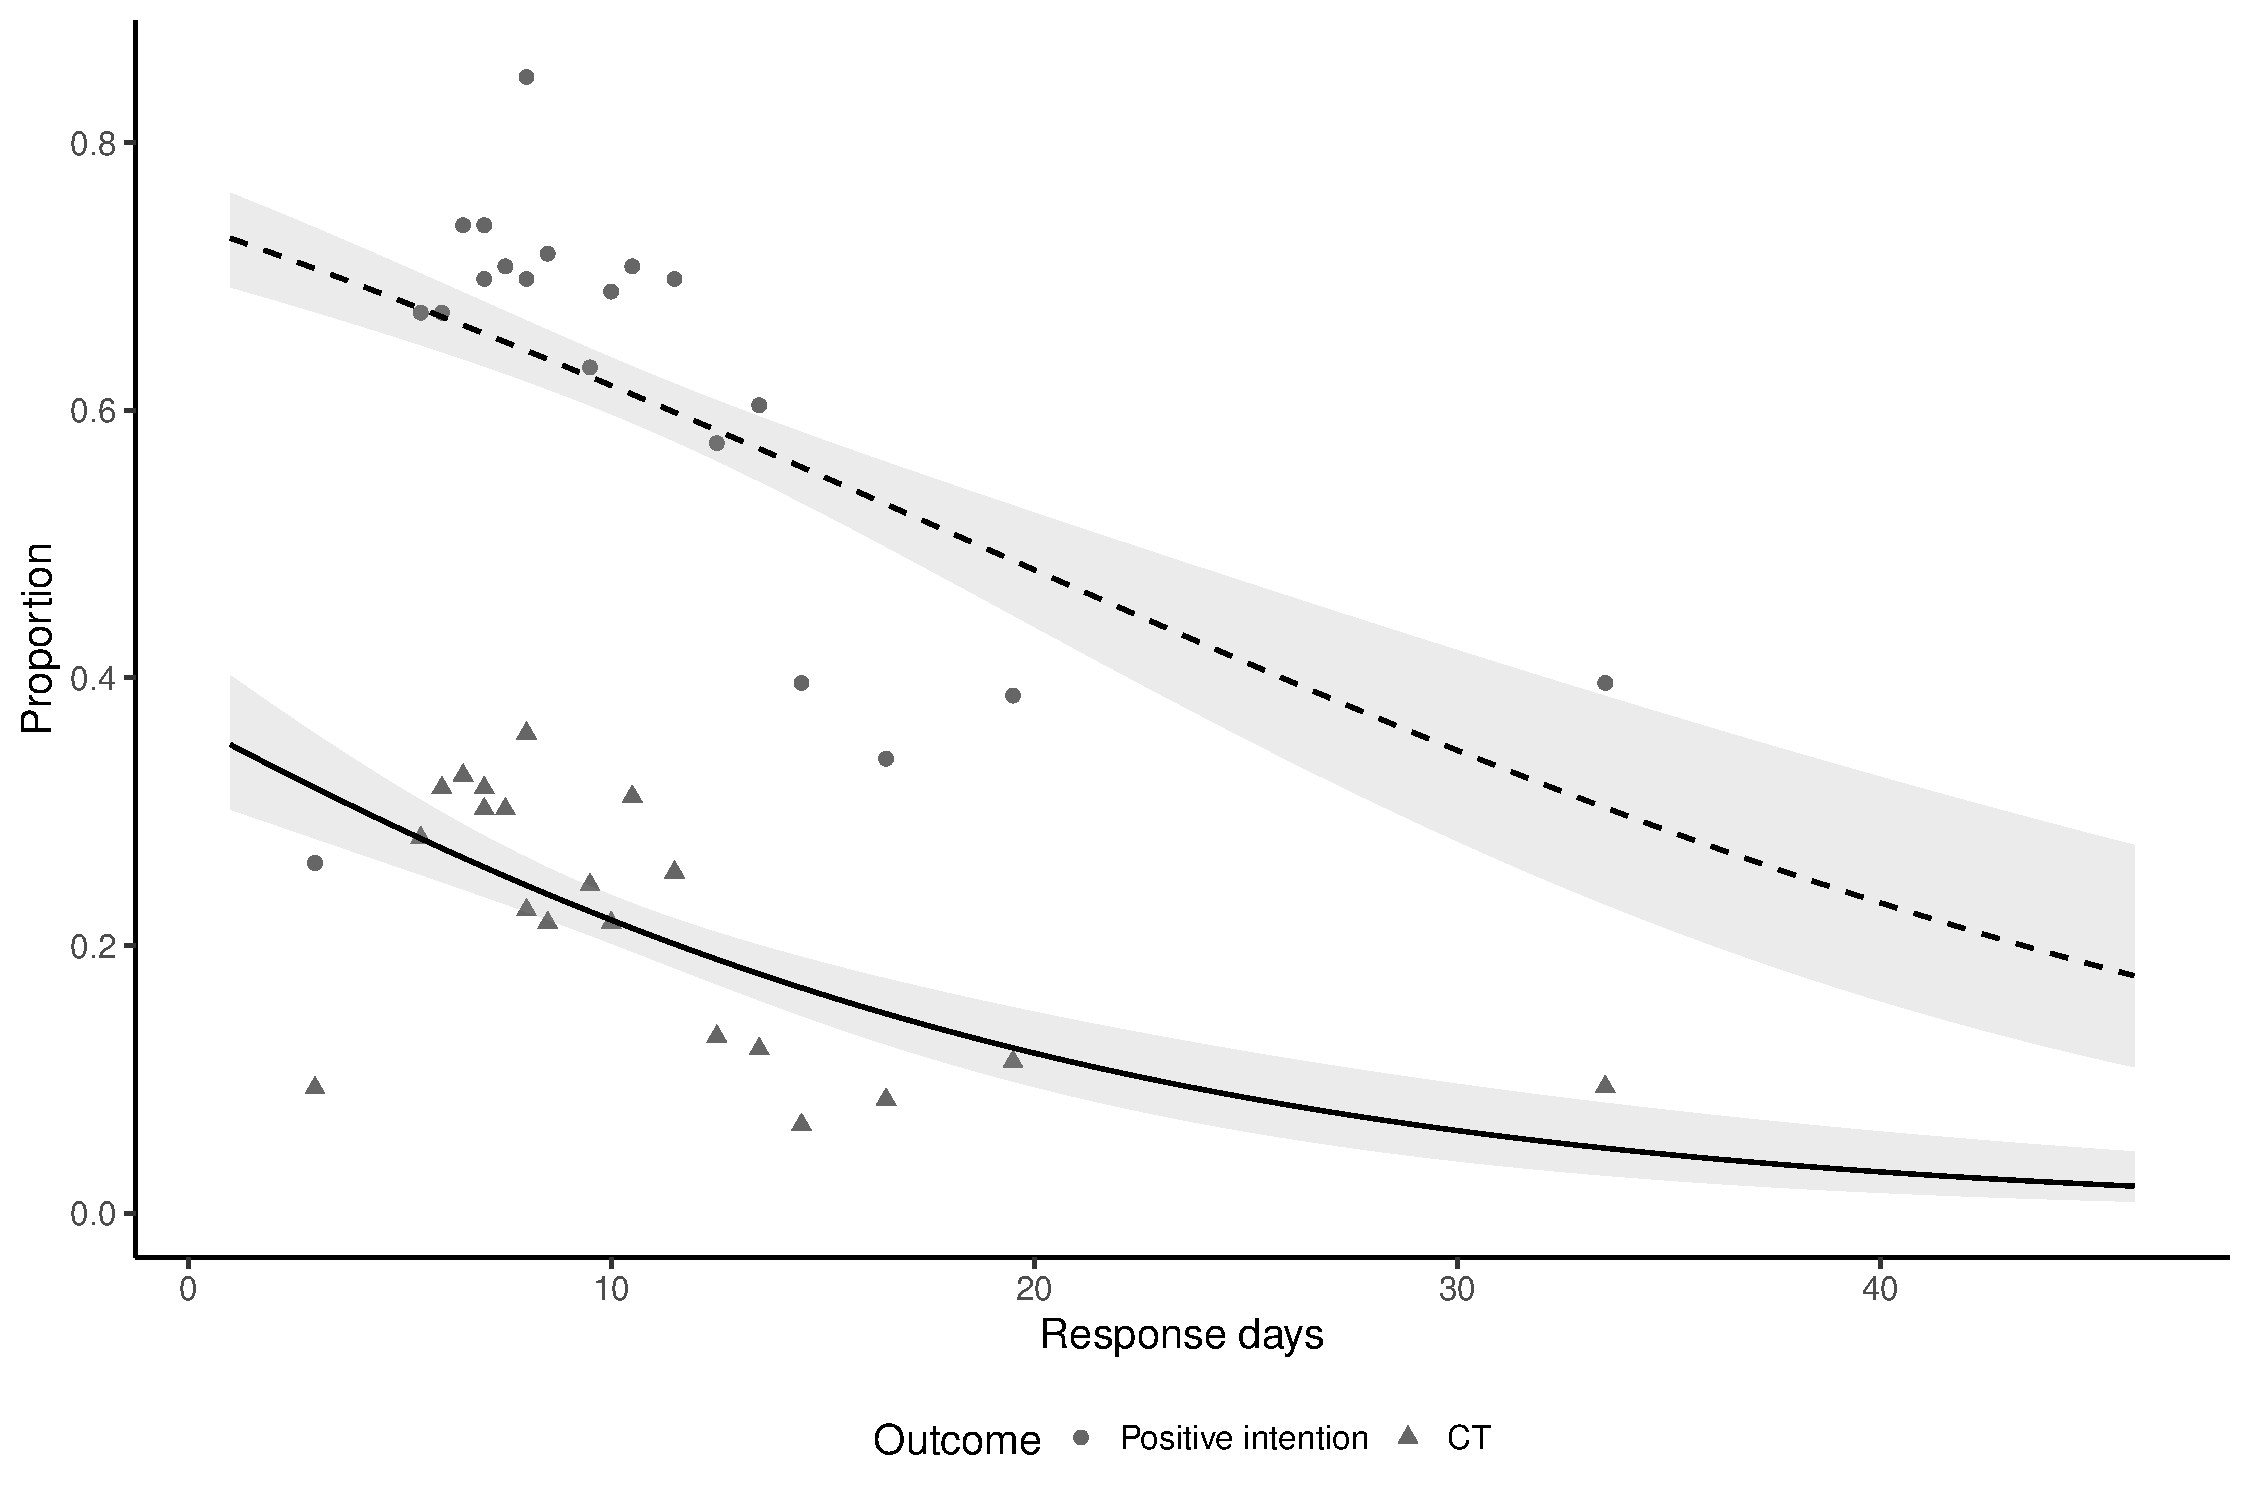
\includegraphics{JMDPRC~4/figure-latex/response-speed-CT-1} \caption{Binned Scatter Plot of CT (or Reply with Positive Intention) vs. Response Days.}\label{fig:response-speed-CT}
\end{figure}

\begin{table}[H]

\caption{\label{tab:test-lm}Linear Probability Model of the CT}
\centering
\fontsize{8}{10}\selectfont
\begin{threeparttable}
\begin{tabular}[t]{lcc}
\toprule
\multicolumn{1}{c}{ } & \multicolumn{2}{c}{CT} \\
\cmidrule(l{3pt}r{3pt}){2-3}
  & (1) & (2)\\
\midrule
Treatment B & \num{3.10}*** & \num{3.18}**\\
 & (\num{1.14}) & (\num{1.27})\\
Treatment C & \num{1.19} & \num{0.88}\\
 & (\num{1.16}) & (\num{1.15})\\
Treatment D & \num{2.39}** & \num{2.63}**\\
 & (\num{1.17}) & (\num{1.16})\\
\midrule
Control average & 22.25 & 22.25\\
Covariates &  & X\\
Num.Obs. & \num{11049} & \num{11049}\\
\bottomrule
\end{tabular}
\begin{tablenotes}
\item \emph{Note}: * $p < 0.1$, ** $p < 0.05$, *** $p < 0.01$. The robust standard errors are in parentheses. The unit of treatment effect is a percentage point. Covariates are gender, (demeaned) age, its squared term, the number of past coordinations, the number of public holidays in the assigned week and the following week, the number of hospitals per 10 square kilometers, the number of hospitals with PBSC collection per 10 square kilometers and the number of hospitals with BM collection per 10 square kilometers. Month and Week FE is month and week (the number of a week within each month) dummy variables. Region represents geographical clusters, where 41 prefectures are grouped into 10 regions, while Hokkaido, Tokyo, Kanagawa, Aichi, Osaka, and Okinawa each form their own region, resulting in 16 region dummies in total. Week (in Dec. and Jan.) consists of dummy variables indicating each week in December 2020 and January 2021 and the remaining period. We controlled winter holidays effect by Region$\times$Week (in Dec. and Jan.) dummies which is the products of these region and week indicators.
\end{tablenotes}
\end{threeparttable}
\end{table}

\begin{table}[H]

\caption{\label{tab:test-logit}Logit Model of the CT}
\centering
\fontsize{8}{10}\selectfont
\begin{threeparttable}
\begin{tabular}[t]{lcc}
\toprule
\multicolumn{1}{c}{ } & \multicolumn{2}{c}{CT} \\
\cmidrule(l{3pt}r{3pt}){2-3}
  & (1) & (2)\\
\midrule
Treatment B & \num{1.19} & \num{1.20}\\
 & {}[\num{1.05}, \num{1.34}] & {}[\num{1.04}, \num{1.38}]\\
Treatment C & \num{1.07} & \num{1.05}\\
 & {}[\num{0.94}, \num{1.22}] & {}[\num{0.93}, \num{1.20}]\\
Treatment D & \num{1.14} & \num{1.16}\\
 & {}[\num{1.01}, \num{1.30}] & {}[\num{1.02}, \num{1.32}]\\
\midrule
Covariates &  & X\\
Num.Obs. & \num{11049} & \num{11049}\\
Log.Lik. & \num{-6083.783} & \num{-5953.670}\\
\bottomrule
\end{tabular}
\begin{tablenotes}
\item \emph{Note}: We show odds ratios and associated 95 percent confidential intervals in square brackets. Covariates are gender, (demeaned) age, its squared term, the number of past coordinations, the number of public holidays in the assigned week and the following week, the number of hospitals per 10 square kilometers, the number of hospitals with PBSC collection per 10 square kilometers and the number of hospitals with BM collection per 10 square kilometers. Month and Week FE is month and week (the number of a week within each month) dummy variables. We controlled winter holidays effect by Region$\times$Week (in Dec. and Jan.) dummies. Region dummies represent geographical clusters, where 41 prefectures are grouped into 10 regions, while Hokkaido, Tokyo, Kanagawa, Aichi, Osaka, and Okinawa each form their own region, resulting in 16 region dummies in total. Week (in Dec. and Jan.) consists of dummy variables indicating each week in December 2020 and January 2021 and the remaining period.
\end{tablenotes}
\end{threeparttable}
\end{table}

\begin{table}[H]

\caption{\label{tab:test-lm-interaction-reg}Heterogenous Message Effects on CT}
\centering
\fontsize{8}{10}\selectfont
\begin{threeparttable}
\begin{tabular}[t]{lcc}
\toprule
\multicolumn{1}{c}{ } & \multicolumn{2}{c}{CT} \\
\cmidrule(l{3pt}r{3pt}){2-3}
  & (1) & (2)\\
\midrule
Treatment B & \num{2.67} & \num{2.28}\\
 & (\num{2.46}) & (\num{2.68})\\
Treatment C & \num{2.64} & \num{1.57}\\
 & (\num{2.49}) & (\num{2.43})\\
Treatment D & \num{5.72}** & \num{5.63}**\\
 & (\num{2.55}) & (\num{2.53})\\
Older female & \num{-0.67} & \num{9.15}\\
 & (\num{2.56}) & (\num{5.89})\\
Young male & \num{4.98}** & \num{2.01}\\
 & (\num{2.39}) & (\num{5.44})\\
Older male & \num{3.62} & \num{11.04}**\\
 & (\num{2.31}) & (\num{5.20})\\
Treatment B $\times$ Older female & \num{0.09} & \num{0.55}\\
 & (\num{3.57}) & (\num{3.92})\\
Treatment C $\times$ Older female & \num{-2.59} & \num{-1.74}\\
 & (\num{3.64}) & (\num{3.61})\\
Treatment D $\times$ Older female & \num{-1.80} & \num{-1.52}\\
 & (\num{3.67}) & (\num{3.66})\\
Treatment B $\times$ Young male & \num{1.13} & \num{0.29}\\
 & (\num{3.27}) & (\num{3.56})\\
Treatment C $\times$ Young male & \num{-3.07} & \num{-1.88}\\
 & (\num{3.27}) & (\num{3.22})\\
Treatment D $\times$ Young male & \num{-7.44}** & \num{-6.99}**\\
 & (\num{3.34}) & (\num{3.30})\\
Treatment B $\times$ Older male & \num{-0.03} & \num{1.98}\\
 & (\num{3.19}) & (\num{3.55})\\
Treatment C $\times$ Older male & \num{-0.41} & \num{0.60}\\
 & (\num{3.27}) & (\num{3.21})\\
Treatment D $\times$ Older male & \num{-2.32} & \num{-1.85}\\
 & (\num{3.31}) & (\num{3.29})\\
\midrule
Covariates &  & X\\
Num.Obs. & \num{11049} & \num{11049}\\
\bottomrule
\end{tabular}
\begin{tablenotes}
\item \emph{Note}: * $p < 0.1$, ** $p < 0.05$, *** $p < 0.01$. The robust standard errors are in parentheses. This tabel tests heterogenous message effects by gender and age. We created two age classes (Younger/Older) based on age 30. Covariates are the number of past coordinations, the number of public holidays in the assigned week and the following week, the number of hospitals per 10 square kilometers, the number of hospitals with PBSC collection per 10 square kilometers and the number of hospitals with BM collection per 10 square kilometers. Month and Week FE is month and week (the number of a week within each month) dummy variables. We controlled winter holidays effect by Region$\times$Week (in Dec. and Jan.) dummies. Region dummies represent geographical clusters, where 41 prefectures are grouped into 10 regions, while Hokkaido, Tokyo, Kanagawa, Aichi, Osaka, and Okinawa each form their own region, resulting in 16 region dummies in total. Week (in Dec. and Jan.) consists of dummy variables indicating each week in December 2020 and January 2021 and the remaining period.
\end{tablenotes}
\end{threeparttable}
\end{table}

\begin{table}[H]

\caption{\label{tab:test-lm-interaction-lh}Linear Combination Test: Message Effects on CT for Specific Gender-Age Group}
\centering
\fontsize{8}{10}\selectfont
\begin{threeparttable}
\begin{tabular}[t]{lcccc}
\toprule
\multicolumn{1}{c}{ } & \multicolumn{2}{c}{Females} & \multicolumn{2}{c}{Males} \\
\cmidrule(l{3pt}r{3pt}){2-3} \cmidrule(l{3pt}r{3pt}){4-5}
\multicolumn{1}{c}{ } & \multicolumn{1}{c}{$\text{Age} < 40$} & \multicolumn{1}{c}{$40 \le \text{Age}$} & \multicolumn{1}{c}{$\text{Age} < 40$} & \multicolumn{1}{c}{$40 \le \text{Age}$} \\
\cmidrule(l{3pt}r{3pt}){2-2} \cmidrule(l{3pt}r{3pt}){3-3} \cmidrule(l{3pt}r{3pt}){4-4} \cmidrule(l{3pt}r{3pt}){5-5}
 & (1) & (2) & (3) & (4)\\
\midrule
Control average & 19.72 & 19.05 & 24.70 & 23.33\\
\addlinespace[0.3em]
\multicolumn{5}{l}{\textbf{Model (1): No covariates}}\\
\hspace{1em}B & 2.67 & 2.76 & 3.80* & 2.64\\
\hspace{1em} & (2.46) & (2.59) & (2.15) & (2.03)\\
\hspace{1em}C & 2.64 & 0.05 & -0.43 & 2.23\\
\hspace{1em} & (2.49) & (2.65) & (2.13) & (2.12)\\
\hspace{1em}D & 5.72** & 3.92 & -1.72 & 3.40\\
\hspace{1em} & (2.55) & (2.64) & (2.16) & (2.12)\\
\addlinespace[0.3em]
\multicolumn{5}{l}{\textbf{Model (2): Including covariates}}\\
\hspace{1em}B & 2.28 & 2.83 & 2.56 & 4.26*\\
\hspace{1em} & (2.68) & (2.86) & (2.34) & (2.33)\\
\hspace{1em}C & 1.57 & -0.17 & -0.31 & 2.17\\
\hspace{1em} & (2.43) & (2.66) & (2.10) & (2.10)\\
\hspace{1em}D & 5.63** & 4.11 & -1.37 & 3.78*\\
\hspace{1em} & (2.53) & (2.65) & (2.12) & (2.10)\\
\bottomrule
\end{tabular}
\begin{tablenotes}
\item \emph{Note}: * $p < 0.1$, ** $p < 0.05$, *** $p < 0.01$. The robust standard errors are in parentheses. We performed a linear combination test on the coefficients of the linear probability model presented in Table \ref{tab:test-lm-interaction-reg}. The null hypothesis for young women is that the treatment dummy is zero. The null hypothesis for the other gender-age groups is that the sum of the treatment dummy and the cross term of the treatment dummy and the gender-age group dummy is zero.
\end{tablenotes}
\end{threeparttable}
\end{table}

\begin{table}[H]

\caption{\label{tab:test-lm-subset1}Subset Regression of CT without Covariates}
\centering
\fontsize{8}{10}\selectfont
\begin{threeparttable}
\begin{tabular}[t]{lcccc}
\toprule
\multicolumn{1}{c}{ } & \multicolumn{4}{c}{CT} \\
\cmidrule(l{3pt}r{3pt}){2-5}
\multicolumn{1}{c}{ } & \multicolumn{2}{c}{Females} & \multicolumn{2}{c}{Males} \\
\cmidrule(l{3pt}r{3pt}){2-3} \cmidrule(l{3pt}r{3pt}){4-5}
\multicolumn{1}{c}{ } & \multicolumn{1}{c}{$\text{Age} < 30$} & \multicolumn{1}{c}{$30 \le \text{Age}$} & \multicolumn{1}{c}{$\text{Age} < 30$} & \multicolumn{1}{c}{$30 \le \text{Age}$} \\
\cmidrule(l{3pt}r{3pt}){2-2} \cmidrule(l{3pt}r{3pt}){3-3} \cmidrule(l{3pt}r{3pt}){4-4} \cmidrule(l{3pt}r{3pt}){5-5}
  & (1) & (2) & (3) & (4)\\
\midrule
Treatment B & \num{2.67} & \num{2.76} & \num{3.80}* & \num{2.64}\\
 & (\num{2.46}) & (\num{2.59}) & (\num{2.15}) & (\num{2.03})\\
Treatment C & \num{2.64} & \num{0.05} & \num{-0.43} & \num{2.23}\\
 & (\num{2.49}) & (\num{2.65}) & (\num{2.12}) & (\num{2.12})\\
Treatment D & \num{5.72}** & \num{3.92} & \num{-1.72} & \num{3.40}\\
 & (\num{2.55}) & (\num{2.64}) & (\num{2.16}) & (\num{2.11})\\
\midrule
Control average & 19.72 & 19.05 & 24.70 & 23.33\\
\addlinespace[0.3em]
\multicolumn{5}{l}{\textit{Multiplicity-adjusted p-values}}\\
\hspace{1em}Treatment B & 0.777 & 0.825 & 0.624 & 0.617\\
\hspace{1em}Treatment C & 0.858 & 0.826 & 0.728 & 0.842\\
\hspace{1em}Treatment D & 0.736 & 0.262 & 0.647 & 0.696\\
Num.Obs. & \num{2268} & \num{1882} & \num{3445} & \num{3454}\\
\bottomrule
\end{tabular}
\begin{tablenotes}
\item \emph{Note}: * $p < 0.1$, ** $p < 0.05$, *** $p < 0.01$. The robust standard errors are in parentheses. We did not control any covariates. Multiplicity-adjusted p-values were calculated with the method proposed by \cite{List2019}.
\end{tablenotes}
\end{threeparttable}
\end{table}

\begin{table}[H]

\caption{\label{tab:test-lm-subset2}Subset Regression of CT with Covariates and Month and Week FE}
\centering
\fontsize{8}{10}\selectfont
\begin{threeparttable}
\begin{tabular}[t]{lcccc}
\toprule
\multicolumn{1}{c}{ } & \multicolumn{4}{c}{CT} \\
\cmidrule(l{3pt}r{3pt}){2-5}
\multicolumn{1}{c}{ } & \multicolumn{2}{c}{Females} & \multicolumn{2}{c}{Males} \\
\cmidrule(l{3pt}r{3pt}){2-3} \cmidrule(l{3pt}r{3pt}){4-5}
\multicolumn{1}{c}{ } & \multicolumn{1}{c}{$\text{Age} < 40$} & \multicolumn{1}{c}{$40 \le \text{Age}$} & \multicolumn{1}{c}{$\text{Age} < 40$} & \multicolumn{1}{c}{$40 \le \text{Age}$} \\
\cmidrule(l{3pt}r{3pt}){2-2} \cmidrule(l{3pt}r{3pt}){3-3} \cmidrule(l{3pt}r{3pt}){4-4} \cmidrule(l{3pt}r{3pt}){5-5}
  & (1) & (2) & (3) & (4)\\
\midrule
Treatment B & \num{2.28} & \num{2.83} & \num{2.56} & \num{4.26}*\\
 & (\num{2.68}) & (\num{2.87}) & (\num{2.34}) & (\num{2.33})\\
Treatment C & \num{1.57} & \num{-0.17} & \num{-0.31} & \num{2.17}\\
 & (\num{2.44}) & (\num{2.66}) & (\num{2.10}) & (\num{2.09})\\
Treatment D & \num{5.63}** & \num{4.11} & \num{-1.37} & \num{3.78}*\\
 & (\num{2.53}) & (\num{2.65}) & (\num{2.12}) & (\num{2.10})\\
\midrule
Control average & 19.72 & 19.05 & 24.70 & 23.33\\
Num.Obs. & \num{2268} & \num{1882} & \num{3445} & \num{3454}\\
\bottomrule
\end{tabular}
\begin{tablenotes}
\item \emph{Note}: * $p < 0.1$, ** $p < 0.05$, *** $p < 0.01$. The robust standard errors are in parentheses. We controlled the number of past coordinations, the number of public holidays in the assigned week and the following week, the number of hospitals per 10 square kilometers, the number of hospitals with PBSC collection per 10 square kilometers and the number of hospitals with BM collection per 10 square kilometers, and month and week (the number of a week within each month) dummy variables.
\end{tablenotes}
\end{threeparttable}
\end{table}

\begin{table}[H]

\caption{\label{tab:test-decompose}Decompose Effect on the CT}
\centering
\fontsize{8}{10}\selectfont
\begin{threeparttable}
\begin{tabular}[t]{lcccccc}
\toprule
\multicolumn{1}{c}{ } & \multicolumn{2}{c}{Positive Intention} & \multicolumn{2}{c}{No exogenous attrition} & \multicolumn{2}{c}{No endogenous attrition} \\
\cmidrule(l{3pt}r{3pt}){2-3} \cmidrule(l{3pt}r{3pt}){4-5} \cmidrule(l{3pt}r{3pt}){6-7}
  & (1) & (2) & (3) & (4) & (5) & (6)\\
\midrule
Treatment B & \num{2.31}* & \num{1.88} & \num{-0.17} & \num{-0.07} & \num{0.97} & \num{1.37}\\
 & (\num{1.33}) & (\num{1.46}) & (\num{0.57}) & (\num{0.61}) & (\num{1.20}) & (\num{1.31})\\
Treatment C & \num{-0.44} & \num{0.20} & \num{-0.93} & \num{-0.95} & \num{2.55}** & \num{1.62}\\
 & (\num{1.37}) & (\num{1.36}) & (\num{0.60}) & (\num{0.60}) & (\num{1.22}) & (\num{1.20})\\
Treatment D & \num{0.59} & \num{0.83} & \num{-0.51} & \num{-0.48} & \num{2.27}* & \num{2.25}*\\
 & (\num{1.37}) & (\num{1.35}) & (\num{0.59}) & (\num{0.59}) & (\num{1.22}) & (\num{1.21})\\
\midrule
Control average & 54.91 & 54.91 & 95.42 & 95.42 & 71.91 & 71.91\\
Covariates &  & X &  & X &  & X\\
Num.Obs. & \num{11049} & \num{11049} & \num{11049} & \num{11049} & \num{11049} & \num{11049}\\
\bottomrule
\end{tabular}
\begin{tablenotes}
\item \emph{Note}: * $p < 0.1$, ** $p < 0.05$, *** $p < 0.01$. The robust standard errors are in parentheses. The outcome ``No exogenous attrition'' is a dummy variable that takes a value of 1 if coordination was not interrupted due to exogenous reasons (patient-side reasons) between reply with positive intention and CT. The outcome ``No endogenous attrition'' is a dummy variable that takes a value of 1 if coordination was not interrupted due to other reasons (mainly donor-side reasons). Covariates are gender, (demeaned) age, its squared term, the number of past coordinations, the number of public holidays in the assigned week and the following week, the number of hospitals per 10 square kilometers, the number of hospitals with PBSC collection per 10 square kilometers and the number of hospitals with BM collection per 10 square kilometers. Month and Week FE is month and week (the number of a week within each month) dummy variables.
\end{tablenotes}
\end{threeparttable}
\end{table}

\begin{table}[H]

\caption{\label{tab:test-decompose-interaction-reg}Heterogenity of Decomposing Effect on the CT}
\centering
\fontsize{8}{10}\selectfont
\begin{threeparttable}
\begin{tabular}[t]{lcccccc}
\toprule
\multicolumn{1}{c}{ } & \multicolumn{2}{c}{Positive Intention} & \multicolumn{2}{c}{No exogenous attrition} & \multicolumn{2}{c}{No endogenous attrition} \\
\cmidrule(l{3pt}r{3pt}){2-3} \cmidrule(l{3pt}r{3pt}){4-5} \cmidrule(l{3pt}r{3pt}){6-7}
  & (1) & (2) & (3) & (4) & (5) & (6)\\
\midrule
Treatment B & \num{-1.90} & \num{-1.45} & \num{1.20} & \num{1.72} & \num{3.38} & \num{2.00}\\
 & (\num{3.03}) & (\num{3.31}) & (\num{1.39}) & (\num{1.43}) & (\num{2.65}) & (\num{2.91})\\
Treatment C & \num{-0.83} & \num{-2.06} & \num{-0.73} & \num{-0.60} & \num{4.20} & \num{4.22}\\
 & (\num{3.06}) & (\num{3.04}) & (\num{1.50}) & (\num{1.50}) & (\num{2.66}) & (\num{2.64})\\
Treatment D & \num{-3.05} & \num{-3.08} & \num{2.12} & \num{2.23}* & \num{6.65}** & \num{6.48}**\\
 & (\num{3.07}) & (\num{3.07}) & (\num{1.35}) & (\num{1.35}) & (\num{2.62}) & (\num{2.62})\\
Older female & \num{7.34}** & \num{9.58} & \num{0.90} & \num{-6.04}* & \num{-8.91}*** & \num{5.61}\\
 & (\num{3.20}) & (\num{7.00}) & (\num{1.49}) & (\num{3.14}) & (\num{3.01}) & (\num{6.38})\\
Young male & \num{-7.03}** & \num{-10.08} & \num{2.99}** & \num{-2.87} & \num{9.02}*** & \num{14.96}***\\
 & (\num{2.90}) & (\num{6.27}) & (\num{1.25}) & (\num{2.73}) & (\num{2.46}) & (\num{5.06})\\
Older male & \num{7.78}*** & \num{8.06} & \num{1.45} & \num{2.05} & \num{-5.62}** & \num{0.90}\\
 & (\num{2.81}) & (\num{6.06}) & (\num{1.30}) & (\num{2.74}) & (\num{2.58}) & (\num{5.37})\\
Treatment B $\times$ Older female & \num{3.99} & \num{2.43} & \num{-0.32} & \num{-2.12} & \num{-3.58} & \num{0.24}\\
 & (\num{4.35}) & (\num{4.80}) & (\num{1.95}) & (\num{2.08}) & (\num{4.07}) & (\num{4.48})\\
Treatment C $\times$ Older female & \num{3.21} & \num{4.48} & \num{-0.76} & \num{-0.92} & \num{-5.04} & \num{-5.30}\\
 & (\num{4.48}) & (\num{4.48}) & (\num{2.19}) & (\num{2.18}) & (\num{4.20}) & (\num{4.20})\\
Treatment D $\times$ Older female & \num{5.26} & \num{5.28} & \num{-2.00} & \num{-2.29} & \num{-5.05} & \num{-4.51}\\
 & (\num{4.40}) & (\num{4.40}) & (\num{1.97}) & (\num{1.96}) & (\num{4.06}) & (\num{4.07})\\
Treatment B $\times$ Young male & \num{7.66}** & \num{6.72} & \num{-2.68} & \num{-3.92}** & \num{-3.85} & \num{-2.51}\\
 & (\num{3.89}) & (\num{4.27}) & (\num{1.67}) & (\num{1.80}) & (\num{3.26}) & (\num{3.59})\\
Treatment C $\times$ Young male & \num{-0.03} & \num{1.28} & \num{-0.41} & \num{-0.48} & \num{-2.63} & \num{-2.67}\\
 & (\num{3.92}) & (\num{3.91}) & (\num{1.76}) & (\num{1.76}) & (\num{3.25}) & (\num{3.24})\\
Treatment D $\times$ Young male & \num{2.74} & \num{2.92} & \num{-4.70}*** & \num{-4.86}*** & \num{-5.48}* & \num{-5.05}\\
 & (\num{3.97}) & (\num{3.96}) & (\num{1.70}) & (\num{1.70}) & (\num{3.25}) & (\num{3.25})\\
Treatment B $\times$ Older male & \num{4.73} & \num{3.06} & \num{-1.58} & \num{-0.75} & \num{-3.17} & \num{-0.32}\\
 & (\num{3.79}) & (\num{4.18}) & (\num{1.72}) & (\num{1.76}) & (\num{3.45}) & (\num{3.82})\\
Treatment C $\times$ Older male & \num{2.47} & \num{3.87} & \num{0.01} & \num{-0.18} & \num{-2.89} & \num{-3.09}\\
 & (\num{3.89}) & (\num{3.88}) & (\num{1.85}) & (\num{1.84}) & (\num{3.52}) & (\num{3.50})\\
Treatment D $\times$ Older male & \num{7.01}* & \num{7.13}* & \num{-2.73} & \num{-2.71} & \num{-6.73}* & \num{-6.38}*\\
 & (\num{3.87}) & (\num{3.87}) & (\num{1.72}) & (\num{1.72}) & (\num{3.48}) & (\num{3.48})\\
\midrule
Covariates &  & X &  & X &  & X\\
Num.Obs. & \num{11049} & \num{11049} & \num{11049} & \num{11049} & \num{11049} & \num{11049}\\
\bottomrule
\end{tabular}
\begin{tablenotes}
\item \emph{Note}: * $p < 0.1$, ** $p < 0.05$, *** $p < 0.01$. The robust standard errors are in parentheses. We created two age classes (Younger/Older) based on age 40. The outcome ``No exogenous attrition'' is a dummy variable that takes a value of 1 if coordination was not interrupted due to exogenous reasons (patient-side reasons) between reply with positive intention and CT. The outcome ``No endogenous attrition'' is a dummy variable that takes a value of 1 if coordination was not interrupted due to other reasons (mainly donor-side reasons). Covariates are the number of past coordinations, the number of public holidays in the assigned week and the following week, the number of hospitals per 10 square kilometers, the number of hospitals with PBSC collection per 10 square kilometers and the number of hospitals with BM collection per 10 square kilometers.
\end{tablenotes}
\end{threeparttable}
\end{table}

\begin{table}[H]

\caption{\label{tab:test-decompose-interaction-lh1}Linear Combination Test: Message Effects on Reply with Positive Intention for Specific Gender-Age Group}
\centering
\fontsize{8}{10}\selectfont
\begin{threeparttable}
\begin{tabular}[t]{lcccc}
\toprule
\multicolumn{1}{c}{ } & \multicolumn{2}{c}{Females} & \multicolumn{2}{c}{Males} \\
\cmidrule(l{3pt}r{3pt}){2-3} \cmidrule(l{3pt}r{3pt}){4-5}
\multicolumn{1}{c}{ } & \multicolumn{1}{c}{$\text{Age} < 40$} & \multicolumn{1}{c}{$40 \le \text{Age}$} & \multicolumn{1}{c}{$\text{Age} < 40$} & \multicolumn{1}{c}{$40 \le \text{Age}$} \\
\cmidrule(l{3pt}r{3pt}){2-2} \cmidrule(l{3pt}r{3pt}){3-3} \cmidrule(l{3pt}r{3pt}){4-4} \cmidrule(l{3pt}r{3pt}){5-5}
 & (1) & (2) & (3) & (4)\\
\midrule
Control average & 53.05 & 60.39 & 46.02 & 60.83\\
\addlinespace[0.3em]
\multicolumn{5}{l}{\textbf{Model (1): No covariates}}\\
\hspace{1em}B & -1.90 & 2.09 & 5.76** & 2.82\\
\hspace{1em} & (3.03) & (3.13) & (2.44) & (2.28)\\
\hspace{1em}C & -0.83 & 2.38 & -0.86 & 1.64\\
\hspace{1em} & (3.06) & (3.28) & (2.46) & (2.40)\\
\hspace{1em}D & -3.05 & 2.21 & -0.31 & 3.96*\\
\hspace{1em} & (3.07) & (3.15) & (2.52) & (2.36)\\
\addlinespace[0.3em]
\multicolumn{5}{l}{\textbf{Model (2): Including covariates}}\\
\hspace{1em}B & -1.45 & 0.99 & 5.27* & 1.61\\
\hspace{1em} & (3.31) & (3.47) & (2.69) & (2.56)\\
\hspace{1em}C & -2.06 & 2.42 & -0.77 & 1.82\\
\hspace{1em} & (3.04) & (3.28) & (2.46) & (2.40)\\
\hspace{1em}D & -3.08 & 2.20 & -0.16 & 4.04*\\
\hspace{1em} & (3.07) & (3.16) & (2.50) & (2.36)\\
\bottomrule
\end{tabular}
\begin{tablenotes}
\item \emph{Note}: * $p < 0.1$, ** $p < 0.05$, *** $p < 0.01$. The robust standard errors are in parentheses. We performed a linear combination test on the coefficients of the linear probability model presented in Table \ref{tab:test-decompose-interaction-reg}. The null hypothesis for young women is that the treatment dummy is zero. The null hypothesis for the other gender-age groups is that the sum of the treatment dummy and the cross term of the treatment dummy and the gender-age group dummy is zero.
\end{tablenotes}
\end{threeparttable}
\end{table}

\begin{table}[H]

\caption{\label{tab:test-decompose-interaction-lh2}Linear Combination Test: Message Effects on No Endogenous Attrition between Reply with Positive Intention and CT for Specific Gender-Age Group}
\centering
\fontsize{8}{10}\selectfont
\begin{threeparttable}
\begin{tabular}[t]{lcccc}
\toprule
\multicolumn{1}{c}{ } & \multicolumn{2}{c}{Females} & \multicolumn{2}{c}{Males} \\
\cmidrule(l{3pt}r{3pt}){2-3} \cmidrule(l{3pt}r{3pt}){4-5}
\multicolumn{1}{c}{ } & \multicolumn{1}{c}{$\text{Age} < 40$} & \multicolumn{1}{c}{$40 \le \text{Age}$} & \multicolumn{1}{c}{$\text{Age} < 40$} & \multicolumn{1}{c}{$40 \le \text{Age}$} \\
\cmidrule(l{3pt}r{3pt}){2-2} \cmidrule(l{3pt}r{3pt}){3-3} \cmidrule(l{3pt}r{3pt}){4-4} \cmidrule(l{3pt}r{3pt}){5-5}
 & (1) & (2) & (3) & (4)\\
\midrule
Control average & 53.05 & 60.39 & 46.02 & 60.83\\
\addlinespace[0.3em]
\multicolumn{5}{l}{\textbf{Model (1): No covariates}}\\
\hspace{1em}B & 3.38 & -0.20 & -0.47 & 0.21\\
\hspace{1em} & (2.65) & (3.09) & (1.90) & (2.21)\\
\hspace{1em}C & 4.20 & -0.85 & 1.57 & 1.31\\
\hspace{1em} & (2.66) & (3.25) & (1.88) & (2.31)\\
\hspace{1em}D & 6.65** & 1.59 & 1.17 & -0.08\\
\hspace{1em} & (2.62) & (3.10) & (1.93) & (2.30)\\
\addlinespace[0.3em]
\multicolumn{5}{l}{\textbf{Model (2): Including covariates}}\\
\hspace{1em}B & 2.00 & 2.24 & -0.51 & 1.68\\
\hspace{1em} & (2.91) & (3.40) & (2.10) & (2.46)\\
\hspace{1em}C & 4.22 & -1.08 & 1.55 & 1.14\\
\hspace{1em} & (2.64) & (3.26) & (1.88) & (2.30)\\
\hspace{1em}D & 6.48** & 1.97 & 1.43 & 0.10\\
\hspace{1em} & (2.62) & (3.11) & (1.93) & (2.30)\\
\bottomrule
\end{tabular}
\begin{tablenotes}
\item \emph{Note}: * $p < 0.1$, ** $p < 0.05$, *** $p < 0.01$. The robust standard errors are in parentheses. We performed a linear combination test on the coefficients of the linear probability model presented in Table \ref{tab:test-decompose-interaction-reg}. The null hypothesis for young women is that the treatment dummy is zero. The null hypothesis for the other gender-age groups is that the sum of the treatment dummy and the cross term of the treatment dummy and the gender-age group dummy is zero.
\end{tablenotes}
\end{threeparttable}
\end{table}

\begin{table}[H]

\caption{\label{tab:coordinate-reg}Linear Probability Model of Coordination}
\centering
\fontsize{8}{10}\selectfont
\begin{threeparttable}
\begin{tabular}[t]{lcccccc}
\toprule
\multicolumn{1}{c}{ } & \multicolumn{2}{c}{Candidate Selection} & \multicolumn{2}{c}{Final Consent} & \multicolumn{2}{c}{Donation} \\
\cmidrule(l{3pt}r{3pt}){2-3} \cmidrule(l{3pt}r{3pt}){4-5} \cmidrule(l{3pt}r{3pt}){6-7}
  & (1) & (2) & (3) & (4) & (5) & (6)\\
\midrule
Treatment B & \num{0.16} & \num{-0.10} & \num{0.26} & \num{-0.01} & \num{0.12} & \num{-0.04}\\
 & (\num{0.65}) & (\num{0.72}) & (\num{0.62}) & (\num{0.68}) & (\num{0.56}) & (\num{0.63})\\
Treatment C & \num{-0.07} & \num{-0.23} & \num{0.06} & \num{-0.07} & \num{0.02} & \num{-0.09}\\
 & (\num{0.66}) & (\num{0.66}) & (\num{0.63}) & (\num{0.63}) & (\num{0.57}) & (\num{0.57})\\
Treatment D & \num{0.50} & \num{0.54} & \num{0.63} & \num{0.67} & \num{0.07} & \num{0.10}\\
 & (\num{0.68}) & (\num{0.68}) & (\num{0.64}) & (\num{0.64}) & (\num{0.57}) & (\num{0.57})\\
\midrule
Control average & 6.19 & 6.19 & 5.44 & 5.44 & 4.50 & 4.50\\
Covariates &  & X &  & X &  & X\\
Num.Obs. & \num{11049} & \num{11049} & \num{11049} & \num{11049} & \num{11049} & \num{11049}\\
\bottomrule
\end{tabular}
\begin{tablenotes}
\item \emph{Note}: * $p < 0.1$, ** $p < 0.05$, *** $p < 0.01$. The robust standard errors are in parentheses. The unit of treatment effect is a percentage point. Individual-level covariates are gender, (demeaned) age, its squared term, the number of past coordinations. Week-level covariates are the number of public holidays in the assigned week and the following week. Prefecture-level covariates are the number of hospitals per 10 square kilometers, the number of hospitals with PBSC collection per 10 square kilometers and the number of hospitals with BM collection per 10 square kilometers. Region represents geographical clusters, where 41 prefectures are grouped into 10 regions, while Hokkaido, Tokyo, Kanagawa, Aichi, Osaka, and Okinawa each form their own region, resulting in 16 region dummies in total. Week (in Dec. and Jan.) consists of dummy variables indicating each week in December 2020 and January 2021 and the remaining period. Region$\times$Week (in Dec. and Jan.) FE represents the products of these region and week indicators.
\end{tablenotes}
\end{threeparttable}
\end{table}

\begin{landscape}\begin{table}[H]

\caption{\label{tab:coordinate-logit}Logit Model of Coordination}
\centering
\fontsize{8}{10}\selectfont
\begin{threeparttable}
\begin{tabular}[t]{lcccccc}
\toprule
\multicolumn{1}{c}{ } & \multicolumn{2}{c}{Candidate Selection} & \multicolumn{2}{c}{Final Consent} & \multicolumn{2}{c}{Donation} \\
\cmidrule(l{3pt}r{3pt}){2-3} \cmidrule(l{3pt}r{3pt}){4-5} \cmidrule(l{3pt}r{3pt}){6-7}
  & (1) & (2) & (3) & (4) & (5) & (6)\\
\midrule
Treatment B & \num{1.03} & \num{0.99} & \num{1.05} & \num{1.00} & \num{1.03} & \num{0.99}\\
 & {}[\num{0.83}, \num{1.28}] & {}[\num{0.77}, \num{1.26}] & {}[\num{0.83}, \num{1.32}] & {}[\num{0.78}, \num{1.30}] & {}[\num{0.80}, \num{1.32}] & {}[\num{0.75}, \num{1.32}]\\
Treatment C & \num{0.99} & \num{0.97} & \num{1.01} & \num{0.99} & \num{1.00} & \num{0.98}\\
 & {}[\num{0.79}, \num{1.24}] & {}[\num{0.77}, \num{1.21}] & {}[\num{0.80}, \num{1.28}] & {}[\num{0.78}, \num{1.26}] & {}[\num{0.77}, \num{1.30}] & {}[\num{0.76}, \num{1.28}]\\
Treatment D & \num{1.09} & \num{1.10} & \num{1.12} & \num{1.13} & \num{1.02} & \num{1.02}\\
 & {}[\num{0.87}, \num{1.35}] & {}[\num{0.88}, \num{1.37}] & {}[\num{0.89}, \num{1.42}] & {}[\num{0.90}, \num{1.43}] & {}[\num{0.78}, \num{1.32}] & {}[\num{0.79}, \num{1.33}]\\
\midrule
Covariates &  & X &  & X &  & X\\
Num.Obs. & \num{11049} & \num{11049} & \num{11049} & \num{11049} & \num{11049} & \num{11049}\\
Log.Lik. & \num{-2610.914} & \num{-2555.918} & \num{-2410.035} & \num{-2357.402} & \num{-2045.363} & \num{-2011.218}\\
\bottomrule
\end{tabular}
\begin{tablenotes}
\item \emph{Note}: We show odds ratios and associated 95 percent confidential intervals in square brackets. Individual-level covariates are gender, (demeaned) age, its squared term, the number of past coordinations. Week-level covariates are the number of public holidays in the assigned week and the following week. Prefecture-level covariates are the number of hospitals per 10 square kilometers, the number of hospitals with PBSC collection per 10 square kilometers and the number of hospitals with BM collection per 10 square kilometers. Region represents geographical clusters, where 41 prefectures are grouped into 10 regions, while Hokkaido, Tokyo, Kanagawa, Aichi, Osaka, and Okinawa each form their own region, resulting in 16 region dummies in total. Week (in Dec. and Jan.) consists of dummy variables indicating each week in December 2020 and January 2021 and the remaining period. Region$\times$Week (in Dec. and Jan.) FE represents the products of these region and week indicators.
\end{tablenotes}
\end{threeparttable}
\end{table}
\end{landscape}

\begin{table}[H]

\caption{\label{tab:consent-lm-interaction-reg}Heterogenous Message Effects on Final Consent}
\centering
\fontsize{8}{10}\selectfont
\begin{threeparttable}
\begin{tabular}[t]{lcc}
\toprule
\multicolumn{1}{c}{ } & \multicolumn{2}{c}{Final Consent} \\
\cmidrule(l{3pt}r{3pt}){2-3}
  & (1) & (2)\\
\midrule
Treatment B & \num{-1.98}* & \num{-2.03}*\\
 & (\num{1.09}) & (\num{1.14})\\
Treatment C & \num{0.68} & \num{0.61}\\
 & (\num{1.28}) & (\num{1.28})\\
Treatment D & \num{-0.64} & \num{-0.61}\\
 & (\num{1.20}) & (\num{1.21})\\
Older female & \num{-1.24} & \num{-1.87}\\
 & (\num{1.21}) & (\num{2.54})\\
Young male & \num{3.02}** & \num{1.83}\\
 & (\num{1.32}) & (\num{2.71})\\
Older male & \num{1.57} & \num{-0.06}\\
 & (\num{1.22}) & (\num{2.45})\\
Treatment B $\times$ Older female & \num{2.29} & \num{1.70}\\
 & (\num{1.57}) & (\num{1.64})\\
Treatment C $\times$ Older female & \num{-0.37} & \num{-0.41}\\
 & (\num{1.74}) & (\num{1.73})\\
Treatment D $\times$ Older female & \num{1.47} & \num{1.31}\\
 & (\num{1.68}) & (\num{1.69})\\
Treatment B $\times$ Young male & \num{3.04}* & \num{2.81}\\
 & (\num{1.71}) & (\num{1.86})\\
Treatment C $\times$ Young male & \num{-1.87} & \num{-1.77}\\
 & (\num{1.78}) & (\num{1.78})\\
Treatment D $\times$ Young male & \num{0.84} & \num{0.88}\\
 & (\num{1.79}) & (\num{1.80})\\
Treatment B $\times$ Older male & \num{2.62}* & \num{2.69}\\
 & (\num{1.57}) & (\num{1.75})\\
Treatment C $\times$ Older male & \num{-0.15} & \num{-0.10}\\
 & (\num{1.74}) & (\num{1.74})\\
Treatment D $\times$ Older male & \num{2.44} & \num{2.48}\\
 & (\num{1.71}) & (\num{1.72})\\
\midrule
Covariates &  & X\\
Num.Obs. & \num{11049} & \num{11049}\\
\bottomrule
\end{tabular}
\begin{tablenotes}
\item \emph{Note}: * $p < 0.1$, ** $p < 0.05$, *** $p < 0.01$. The robust standard errors are in parentheses. This tabel tests heterogenous message effects by gender and age. We created two age classes (Younger/Older) based on age 30. Covariates are the number of past coordinations, the number of public holidays in the assigned week and the following week, the number of hospitals per 10 square kilometers, the number of hospitals with PBSC collection per 10 square kilometers and the number of hospitals with BM collection per 10 square kilometers. Month and Week FE is month and week (the number of a week within each month) dummy variables. We controlled winter holidays effect by Region$\times$Week (in Dec. and Jan.) dummies. Region dummies represent geographical clusters, where 41 prefectures are grouped into 10 regions, while Hokkaido, Tokyo, Kanagawa, Aichi, Osaka, and Okinawa each form their own region, resulting in 16 region dummies in total. Week (in Dec. and Jan.) consists of dummy variables indicating each week in December 2020 and January 2021 and the remaining period.
\end{tablenotes}
\end{threeparttable}
\end{table}

\begin{table}[H]

\caption{\label{tab:consent-lm-interaction-lh}Linear Combination Test: Message Effects on Final Consent for Specific Gender-Age Group}
\centering
\fontsize{8}{10}\selectfont
\begin{threeparttable}
\begin{tabular}[t]{lcccc}
\toprule
\multicolumn{1}{c}{ } & \multicolumn{2}{c}{Females} & \multicolumn{2}{c}{Males} \\
\cmidrule(l{3pt}r{3pt}){2-3} \cmidrule(l{3pt}r{3pt}){4-5}
\multicolumn{1}{c}{ } & \multicolumn{1}{c}{$\text{Age} < 40$} & \multicolumn{1}{c}{$40 \le \text{Age}$} & \multicolumn{1}{c}{$\text{Age} < 40$} & \multicolumn{1}{c}{$40 \le \text{Age}$} \\
\cmidrule(l{3pt}r{3pt}){2-2} \cmidrule(l{3pt}r{3pt}){3-3} \cmidrule(l{3pt}r{3pt}){4-4} \cmidrule(l{3pt}r{3pt}){5-5}
 & (1) & (2) & (3) & (4)\\
\midrule
Control average & 4.27 & 3.03 & 7.29 & 5.83\\
\addlinespace[0.3em]
\multicolumn{5}{l}{\textbf{Model (1): No covariates}}\\
\hspace{1em}B & -1.98* & 0.31 & 1.06 & 0.63\\
\hspace{1em} & (1.09) & (1.13) & (1.31) & (1.13)\\
\hspace{1em}C & 0.68 & 0.31 & -1.19 & 0.53\\
\hspace{1em} & (1.28) & (1.19) & (1.24) & (1.18)\\
\hspace{1em}D & -0.64 & 0.83 & 0.21 & 1.80\\
\hspace{1em} & (1.20) & (1.18) & (1.32) & (1.22)\\
\addlinespace[0.3em]
\multicolumn{5}{l}{\textbf{Model (2): Including covariates}}\\
\hspace{1em}B & -2.03* & -0.33 & 0.77 & 0.65\\
\hspace{1em} & (1.14) & (1.17) & (1.46) & (1.32)\\
\hspace{1em}C & 0.61 & 0.19 & -1.17 & 0.51\\
\hspace{1em} & (1.28) & (1.17) & (1.24) & (1.18)\\
\hspace{1em}D & -0.61 & 0.70 & 0.27 & 1.87\\
\hspace{1em} & (1.21) & (1.18) & (1.33) & (1.22)\\
\bottomrule
\end{tabular}
\begin{tablenotes}
\item \emph{Note}: * $p < 0.1$, ** $p < 0.05$, *** $p < 0.01$. The robust standard errors are in parentheses. We performed a linear combination test on the coefficients of the linear probability model presented in Table \ref{tab:consent-lm-interaction-reg}. The null hypothesis for young women is that the treatment dummy is zero. The null hypothesis for the other gender-age groups is that the sum of the treatment dummy and the cross term of the treatment dummy and the gender-age group dummy is zero.
\end{tablenotes}
\end{threeparttable}
\end{table}

\begin{table}[H]

\caption{\label{tab:consent-lm-subset1}Subset Regression of Final Consent without Covariates}
\centering
\fontsize{8}{10}\selectfont
\begin{threeparttable}
\begin{tabular}[t]{lcccc}
\toprule
\multicolumn{1}{c}{ } & \multicolumn{4}{c}{CT} \\
\cmidrule(l{3pt}r{3pt}){2-5}
\multicolumn{1}{c}{ } & \multicolumn{2}{c}{Females} & \multicolumn{2}{c}{Males} \\
\cmidrule(l{3pt}r{3pt}){2-3} \cmidrule(l{3pt}r{3pt}){4-5}
\multicolumn{1}{c}{ } & \multicolumn{1}{c}{$\text{Age} < 30$} & \multicolumn{1}{c}{$30 \le \text{Age}$} & \multicolumn{1}{c}{$\text{Age} < 30$} & \multicolumn{1}{c}{$30 \le \text{Age}$} \\
\cmidrule(l{3pt}r{3pt}){2-2} \cmidrule(l{3pt}r{3pt}){3-3} \cmidrule(l{3pt}r{3pt}){4-4} \cmidrule(l{3pt}r{3pt}){5-5}
  & (1) & (2) & (3) & (4)\\
\midrule
Treatment B & \num{-1.98}* & \num{0.31} & \num{1.06} & \num{0.63}\\
 & (\num{1.09}) & (\num{1.13}) & (\num{1.31}) & (\num{1.13})\\
Treatment C & \num{0.68} & \num{0.31} & \num{-1.19} & \num{0.53}\\
 & (\num{1.28}) & (\num{1.19}) & (\num{1.24}) & (\num{1.18})\\
Treatment D & \num{-0.64} & \num{0.83} & \num{0.21} & \num{1.80}\\
 & (\num{1.20}) & (\num{1.18}) & (\num{1.32}) & (\num{1.22})\\
\midrule
Control average & 4.27 & 3.03 & 7.29 & 5.83\\
\addlinespace[0.3em]
\multicolumn{5}{l}{\textit{Multiplicity-adjusted p-values}}\\
\hspace{1em}Treatment B & 0.882 & 0.974 & 0.982 & 0.994\\
\hspace{1em}Treatment C & 0.873 & 0.990 & 0.957 & 0.982\\
\hspace{1em}Treatment D & 0.984 & 0.987 & 0.982 & 0.979\\
Num.Obs. & \num{2268} & \num{1882} & \num{3445} & \num{3454}\\
\bottomrule
\end{tabular}
\begin{tablenotes}
\item \emph{Note}: * $p < 0.1$, ** $p < 0.05$, *** $p < 0.01$. The robust standard errors are in parentheses. We did not control any covariates. Multiplicity-adjusted p-values were calculated with the method proposed by \cite{List2019}.
\end{tablenotes}
\end{threeparttable}
\end{table}

\begin{table}[H]

\caption{\label{tab:consent-lm-subset2}Subset Regression of Final Consent with Covariates and Month and Week FE}
\centering
\fontsize{8}{10}\selectfont
\begin{threeparttable}
\begin{tabular}[t]{lcccc}
\toprule
\multicolumn{1}{c}{ } & \multicolumn{4}{c}{Final Consent} \\
\cmidrule(l{3pt}r{3pt}){2-5}
\multicolumn{1}{c}{ } & \multicolumn{2}{c}{Females} & \multicolumn{2}{c}{Males} \\
\cmidrule(l{3pt}r{3pt}){2-3} \cmidrule(l{3pt}r{3pt}){4-5}
\multicolumn{1}{c}{ } & \multicolumn{1}{c}{$\text{Age} < 40$} & \multicolumn{1}{c}{$40 \le \text{Age}$} & \multicolumn{1}{c}{$\text{Age} < 40$} & \multicolumn{1}{c}{$40 \le \text{Age}$} \\
\cmidrule(l{3pt}r{3pt}){2-2} \cmidrule(l{3pt}r{3pt}){3-3} \cmidrule(l{3pt}r{3pt}){4-4} \cmidrule(l{3pt}r{3pt}){5-5}
  & (1) & (2) & (3) & (4)\\
\midrule
Treatment B & \num{-2.03}* & \num{-0.33} & \num{0.77} & \num{0.65}\\
 & (\num{1.14}) & (\num{1.17}) & (\num{1.46}) & (\num{1.32})\\
Treatment C & \num{0.61} & \num{0.19} & \num{-1.17} & \num{0.51}\\
 & (\num{1.28}) & (\num{1.17}) & (\num{1.24}) & (\num{1.18})\\
Treatment D & \num{-0.61} & \num{0.70} & \num{0.27} & \num{1.87}\\
 & (\num{1.21}) & (\num{1.19}) & (\num{1.33}) & (\num{1.22})\\
\midrule
Control average & 4.27 & 3.03 & 7.29 & 5.83\\
Num.Obs. & \num{2268} & \num{1882} & \num{3445} & \num{3454}\\
\bottomrule
\end{tabular}
\begin{tablenotes}
\item \emph{Note}: * $p < 0.1$, ** $p < 0.05$, *** $p < 0.01$. The robust standard errors are in parentheses. We controlled the number of past coordinations, the number of public holidays in the assigned week and the following week, the number of hospitals per 10 square kilometers, the number of hospitals with PBSC collection per 10 square kilometers and the number of hospitals with BM collection per 10 square kilometers, and month and week (the number of a week within each month) dummy variables.
\end{tablenotes}
\end{threeparttable}
\end{table}

\begin{table}[H]

\caption{\label{tab:lm-test-initial-matched}Linear Probability Model of the CT (Only Initial Matched Candidates)}
\centering
\fontsize{8}{10}\selectfont
\begin{threeparttable}
\begin{tabular}[t]{lcc}
\toprule
\multicolumn{1}{c}{ } & \multicolumn{2}{c}{CT} \\
\cmidrule(l{3pt}r{3pt}){2-3}
  & (1) & (2)\\
\midrule
Treatment B & \num{2.51}* & \num{1.84}\\
 & (\num{1.34}) & (\num{1.51})\\
Treatment C & \num{-0.83} & \num{-0.93}\\
 & (\num{1.35}) & (\num{1.35})\\
Treatment D & \num{1.94} & \num{1.93}\\
 & (\num{1.36}) & (\num{1.37})\\
\midrule
Control average & 18.67 & 18.67\\
Covariates &  & X\\
Num.Obs. & \num{7016} & \num{7016}\\
\bottomrule
\end{tabular}
\begin{tablenotes}
\item \emph{Note}: * $p < 0.1$, ** $p < 0.05$, *** $p < 0.01$. The robust standard errors are in parentheses. The unit of treatment effect is a percentage point. Individual-level covariates are gender, (demeaned) age, its squared term, the number of past coordinations. Week-level covariates are the number of public holidays in the assigned week and the following week. Prefecture-level covariates are the number of hospitals per 10 square kilometers, the number of hospitals with PBSC collection per 10 square kilometers and the number of hospitals with BM collection per 10 square kilometers. Region represents geographical clusters, where 41 prefectures are grouped into 10 regions, while Hokkaido, Tokyo, Kanagawa, Aichi, Osaka, and Okinawa each form their own region, resulting in 16 region dummies in total. Week (in Dec. and Jan.) consists of dummy variables indicating each week in December 2020 and January 2021 and the remaining period. Region$\times$Week (in Dec. and Jan.) FE represents the products of these region and week indicators.
\end{tablenotes}
\end{threeparttable}
\end{table}

\begin{landscape}\begin{table}[H]

\caption{\label{tab:logit-test-initial-matched}Logit Model of the CT (Only Initial Matched Candidates)}
\centering
\fontsize{8}{10}\selectfont
\begin{threeparttable}
\begin{tabular}[t]{lcc}
\toprule
\multicolumn{1}{c}{ } & \multicolumn{2}{c}{CT} \\
\cmidrule(l{3pt}r{3pt}){2-3}
  & (1) & (2)\\
\midrule
Treatment B & \num{1.17} & \num{1.12}\\
 & {}[\num{0.99}, \num{1.38}] & {}[\num{0.93}, \num{1.35}]\\
Treatment C & \num{0.95} & \num{0.94}\\
 & {}[\num{0.79}, \num{1.13}] & {}[\num{0.79}, \num{1.12}]\\
Treatment D & \num{1.13} & \num{1.13}\\
 & {}[\num{0.95}, \num{1.34}] & {}[\num{0.95}, \num{1.34}]\\
\midrule
Covariates &  & X\\
Num.Obs. & \num{7016} & \num{7016}\\
Log.Lik. & \num{-3472.809} & \num{-3460.764}\\
\bottomrule
\end{tabular}
\begin{tablenotes}
\item \emph{Note}: We show odds ratios and associated 95 percent confidential intervals in square brackets. Individual-level covariates are gender, (demeaned) age, its squared term, the number of past coordinations. Week-level covariates are the number of public holidays in the assigned week and the following week. Prefecture-level covariates are the number of hospitals per 10 square kilometers, the number of hospitals with PBSC collection per 10 square kilometers and the number of hospitals with BM collection per 10 square kilometers. Region represents geographical clusters, where 41 prefectures are grouped into 10 regions, while Hokkaido, Tokyo, Kanagawa, Aichi, Osaka, and Okinawa each form their own region, resulting in 16 region dummies in total. Week (in Dec. and Jan.) consists of dummy variables indicating each week in December 2020 and January 2021 and the remaining period. Region$\times$Week (in Dec. and Jan.) FE represents the products of these region and week indicators.
\end{tablenotes}
\end{threeparttable}
\end{table}
\end{landscape}

\begin{table}[H]

\caption{\label{tab:lm-test-interaction-init-reg}Heterogenous Message Effects on CT (Only Initially Matched Candidates)}
\centering
\fontsize{8}{10}\selectfont
\begin{threeparttable}
\begin{tabular}[t]{lcc}
\toprule
\multicolumn{1}{c}{ } & \multicolumn{2}{c}{CT} \\
\cmidrule(l{3pt}r{3pt}){2-3}
  & (1) & (2)\\
\midrule
Treatment B & \num{1.43} & \num{0.04}\\
 & (\num{2.71}) & (\num{2.97})\\
Treatment C & \num{-3.03} & \num{-3.28}\\
 & (\num{2.61}) & (\num{2.61})\\
Treatment D & \num{2.57} & \num{2.30}\\
 & (\num{2.74}) & (\num{2.76})\\
Older female & \num{-0.07} & \num{1.61}\\
 & (\num{2.96}) & (\num{6.20})\\
Young male & \num{4.40} & \num{3.56}\\
 & (\num{2.71}) & (\num{5.53})\\
Older male & \num{-1.54} & \num{5.59}\\
 & (\num{2.63}) & (\num{5.54})\\
Treatment B $\times$ Older female & \num{-2.09} & \num{-1.54}\\
 & (\num{4.09}) & (\num{4.49})\\
Treatment C $\times$ Older female & \num{2.72} & \num{2.69}\\
 & (\num{4.16}) & (\num{4.17})\\
Treatment D $\times$ Older female & \num{1.71} & \num{1.60}\\
 & (\num{4.19}) & (\num{4.21})\\
Treatment B $\times$ Young male & \num{0.10} & \num{-0.04}\\
 & (\num{3.70}) & (\num{4.10})\\
Treatment C $\times$ Young male & \num{-0.14} & \num{0.41}\\
 & (\num{3.59}) & (\num{3.59})\\
Treatment D $\times$ Young male & \num{-6.55}* & \num{-6.25}*\\
 & (\num{3.70}) & (\num{3.71})\\
Treatment B $\times$ Older male & \num{4.64} & \num{7.67}*\\
 & (\num{3.69}) & (\num{4.21})\\
Treatment C $\times$ Older male & \num{6.47}* & \num{6.77}*\\
 & (\num{3.72}) & (\num{3.71})\\
Treatment D $\times$ Older male & \num{4.20} & \num{4.89}\\
 & (\num{3.82}) & (\num{3.85})\\
\midrule
Covariates &  & X\\
Num.Obs. & \num{7016} & \num{7016}\\
\bottomrule
\end{tabular}
\begin{tablenotes}
\item \emph{Note}: * $p < 0.1$, ** $p < 0.05$, *** $p < 0.01$. The robust standard errors are in parentheses. This tabel tests heterogenous message effects by gender and age. We created two age classes (Younger/Older) based on age 30. Covariates are the number of past coordinations, the number of public holidays in the assigned week and the following week, the number of hospitals per 10 square kilometers, the number of hospitals with PBSC collection per 10 square kilometers and the number of hospitals with BM collection per 10 square kilometers. Month and Week FE is month and week (the number of a week within each month) dummy variables. We controlled winter holidays effect by Region$\times$Week (in Dec. and Jan.) dummies. Region dummies represent geographical clusters, where 41 prefectures are grouped into 10 regions, while Hokkaido, Tokyo, Kanagawa, Aichi, Osaka, and Okinawa each form their own region, resulting in 16 region dummies in total. Week (in Dec. and Jan.) consists of dummy variables indicating each week in December 2020 and January 2021 and the remaining period.
\end{tablenotes}
\end{threeparttable}
\end{table}

\begin{table}[H]

\caption{\label{tab:lm-test-interaction-init-lh}Linear Combination Test: Message Effects on CT for Specific Gender-Age Group (Only Initially Matched Candidates)}
\centering
\fontsize{8}{10}\selectfont
\begin{threeparttable}
\begin{tabular}[t]{lcccc}
\toprule
\multicolumn{1}{c}{ } & \multicolumn{2}{c}{Females} & \multicolumn{2}{c}{Males} \\
\cmidrule(l{3pt}r{3pt}){2-3} \cmidrule(l{3pt}r{3pt}){4-5}
\multicolumn{1}{c}{ } & \multicolumn{1}{c}{$\text{Age} < 40$} & \multicolumn{1}{c}{$40 \le \text{Age}$} & \multicolumn{1}{c}{$\text{Age} < 40$} & \multicolumn{1}{c}{$40 \le \text{Age}$} \\
\cmidrule(l{3pt}r{3pt}){2-2} \cmidrule(l{3pt}r{3pt}){3-3} \cmidrule(l{3pt}r{3pt}){4-4} \cmidrule(l{3pt}r{3pt}){5-5}
 & (1) & (2) & (3) & (4)\\
\midrule
Control average & 17.75 & 17.69 & 22.15 & 16.21\\
\addlinespace[0.3em]
\multicolumn{5}{l}{\textbf{Model (1): No covariates}}\\
\hspace{1em}B & 1.43 & -0.65 & 1.53 & 6.07**\\
\hspace{1em} & (2.71) & (3.07) & (2.53) & (2.50)\\
\hspace{1em}C & -3.03 & -0.31 & -3.16 & 3.45\\
\hspace{1em} & (2.61) & (3.24) & (2.47) & (2.65)\\
\hspace{1em}D & 2.57 & 4.27 & -3.99 & 6.76**\\
\hspace{1em} & (2.74) & (3.17) & (2.48) & (2.67)\\
\addlinespace[0.3em]
\multicolumn{5}{l}{\textbf{Model (2): Including covariates}}\\
\hspace{1em}B & 0.04 & -1.50 & 0.01 & 7.71***\\
\hspace{1em} & (2.97) & (3.37) & (2.83) & (2.99)\\
\hspace{1em}C & -3.28 & -0.59 & -2.87 & 3.49\\
\hspace{1em} & (2.61) & (3.25) & (2.47) & (2.65)\\
\hspace{1em}D & 2.30 & 3.89 & -3.95 & 7.18***\\
\hspace{1em} & (2.76) & (3.19) & (2.47) & (2.68)\\
\bottomrule
\end{tabular}
\begin{tablenotes}
\item \emph{Note}: * $p < 0.1$, ** $p < 0.05$, *** $p < 0.01$. The robust standard errors are in parentheses. We performed a linear combination test on the coefficients of the linear probability model presented in Table \ref{tab:lm-test-interaction-init-reg}. The null hypothesis for young women is that the treatment dummy is zero. The null hypothesis for the other gender-age groups is that the sum of the treatment dummy and the cross term of the treatment dummy and the gender-age group dummy is zero.
\end{tablenotes}
\end{threeparttable}
\end{table}

\begin{table}[H]

\caption{\label{tab:lm-test-subset1-init}Subset Regression of CT without Covariates (Only Initially Matched Candidates)}
\centering
\fontsize{8}{10}\selectfont
\begin{threeparttable}
\begin{tabular}[t]{lcccc}
\toprule
\multicolumn{1}{c}{ } & \multicolumn{4}{c}{CT} \\
\cmidrule(l{3pt}r{3pt}){2-5}
\multicolumn{1}{c}{ } & \multicolumn{2}{c}{Females} & \multicolumn{2}{c}{Males} \\
\cmidrule(l{3pt}r{3pt}){2-3} \cmidrule(l{3pt}r{3pt}){4-5}
\multicolumn{1}{c}{ } & \multicolumn{1}{c}{$\text{Age} < 30$} & \multicolumn{1}{c}{$30 \le \text{Age}$} & \multicolumn{1}{c}{$\text{Age} < 30$} & \multicolumn{1}{c}{$30 \le \text{Age}$} \\
\cmidrule(l{3pt}r{3pt}){2-2} \cmidrule(l{3pt}r{3pt}){3-3} \cmidrule(l{3pt}r{3pt}){4-4} \cmidrule(l{3pt}r{3pt}){5-5}
  & (1) & (2) & (3) & (4)\\
\midrule
Treatment B & \num{1.43} & \num{-0.65} & \num{1.53} & \num{6.07}**\\
 & (\num{2.71}) & (\num{3.07}) & (\num{2.53}) & (\num{2.50})\\
Treatment C & \num{-3.03} & \num{-0.31} & \num{-3.16} & \num{3.45}\\
 & (\num{2.61}) & (\num{3.24}) & (\num{2.47}) & (\num{2.65})\\
Treatment D & \num{2.57} & \num{4.27} & \num{-3.99} & \num{6.76}**\\
 & (\num{2.74}) & (\num{3.17}) & (\num{2.48}) & (\num{2.66})\\
\midrule
Control average & 17.75 & 17.69 & 22.15 & 16.21\\
\addlinespace[0.3em]
\multicolumn{5}{l}{\textit{Multiplicity-adjusted p-values}}\\
\hspace{1em}Treatment B & 0.777 & 0.825 & 0.624 & 0.617\\
\hspace{1em}Treatment C & 0.858 & 0.826 & 0.728 & 0.842\\
\hspace{1em}Treatment D & 0.736 & 0.262 & 0.647 & 0.696\\
Num.Obs. & \num{1685} & \num{1207} & \num{2283} & \num{1841}\\
\bottomrule
\end{tabular}
\begin{tablenotes}
\item \emph{Note}: * $p < 0.1$, ** $p < 0.05$, *** $p < 0.01$. The robust standard errors are in parentheses. We did not control any covariates. Multiplicity-adjusted p-values were calculated with the method proposed by \cite{List2019}.
\end{tablenotes}
\end{threeparttable}
\end{table}

\begin{table}[H]

\caption{\label{tab:lm-test-subset2-init}Subset Regression of CT with Covariates and Month and Week FE (Only Initially Matched Candidates)}
\centering
\fontsize{8}{10}\selectfont
\begin{threeparttable}
\begin{tabular}[t]{lcccc}
\toprule
\multicolumn{1}{c}{ } & \multicolumn{4}{c}{CT} \\
\cmidrule(l{3pt}r{3pt}){2-5}
\multicolumn{1}{c}{ } & \multicolumn{2}{c}{Females} & \multicolumn{2}{c}{Males} \\
\cmidrule(l{3pt}r{3pt}){2-3} \cmidrule(l{3pt}r{3pt}){4-5}
\multicolumn{1}{c}{ } & \multicolumn{1}{c}{$\text{Age} < 40$} & \multicolumn{1}{c}{$40 \le \text{Age}$} & \multicolumn{1}{c}{$\text{Age} < 40$} & \multicolumn{1}{c}{$40 \le \text{Age}$} \\
\cmidrule(l{3pt}r{3pt}){2-2} \cmidrule(l{3pt}r{3pt}){3-3} \cmidrule(l{3pt}r{3pt}){4-4} \cmidrule(l{3pt}r{3pt}){5-5}
  & (1) & (2) & (3) & (4)\\
\midrule
Treatment B & \num{0.04} & \num{-1.50} & \num{0.01} & \num{7.71}***\\
 & (\num{2.97}) & (\num{3.37}) & (\num{2.83}) & (\num{2.99})\\
Treatment C & \num{-3.28} & \num{-0.59} & \num{-2.87} & \num{3.49}\\
 & (\num{2.61}) & (\num{3.26}) & (\num{2.47}) & (\num{2.65})\\
Treatment D & \num{2.30} & \num{3.89} & \num{-3.95} & \num{7.18}***\\
 & (\num{2.76}) & (\num{3.19}) & (\num{2.47}) & (\num{2.68})\\
\midrule
Control average & 17.75 & 17.69 & 22.15 & 16.21\\
Num.Obs. & \num{1685} & \num{1207} & \num{2283} & \num{1841}\\
\bottomrule
\end{tabular}
\begin{tablenotes}
\item \emph{Note}: * $p < 0.1$, ** $p < 0.05$, *** $p < 0.01$. The robust standard errors are in parentheses. We controlled the number of past coordinations, the number of public holidays in the assigned week and the following week, the number of hospitals per 10 square kilometers, the number of hospitals with PBSC collection per 10 square kilometers and the number of hospitals with BM collection per 10 square kilometers, and month and week (the number of a week within each month) dummy variables.
\end{tablenotes}
\end{threeparttable}
\end{table}

\begin{table}[H]

\caption{\label{tab:test-decompose-init}Decompose Effect on the CT (Only Intially Matched Candidates)}
\centering
\fontsize{8}{10}\selectfont
\begin{threeparttable}
\begin{tabular}[t]{lcccccc}
\toprule
\multicolumn{1}{c}{ } & \multicolumn{2}{c}{Positive Intention} & \multicolumn{2}{c}{No exogenous attrition} & \multicolumn{2}{c}{No endogenous attrition} \\
\cmidrule(l{3pt}r{3pt}){2-3} \cmidrule(l{3pt}r{3pt}){4-5} \cmidrule(l{3pt}r{3pt}){6-7}
  & (1) & (2) & (3) & (4) & (5) & (6)\\
\midrule
Treatment B & \num{2.95}* & \num{1.50} & \num{-0.24} & \num{-0.11} & \num{-0.21} & \num{0.46}\\
 & (\num{1.68}) & (\num{1.85}) & (\num{0.74}) & (\num{0.79}) & (\num{1.55}) & (\num{1.70})\\
Treatment C & \num{-1.79} & \num{-1.09} & \num{-0.61} & \num{-0.65} & \num{1.57} & \num{0.80}\\
 & (\num{1.74}) & (\num{1.72}) & (\num{0.78}) & (\num{0.77}) & (\num{1.59}) & (\num{1.56})\\
Treatment D & \num{-0.44} & \num{-0.45} & \num{0.16} & \num{0.15} & \num{2.16} & \num{2.17}\\
 & (\num{1.72}) & (\num{1.68}) & (\num{0.74}) & (\num{0.74}) & (\num{1.56}) & (\num{1.54})\\
\midrule
Control average & 53.52 & 53.52 & 95.08 & 95.08 & 70.07 & 70.07\\
Covariates &  & X &  & X &  & X\\
Num.Obs. & \num{7016} & \num{7016} & \num{7016} & \num{7016} & \num{7016} & \num{7016}\\
\bottomrule
\end{tabular}
\begin{tablenotes}
\item \emph{Note}: * $p < 0.1$, ** $p < 0.05$, *** $p < 0.01$. The robust standard errors are in parentheses. The outcome ``No exogenous attrition'' is a dummy variable that takes a value of 1 if coordination was not interrupted due to exogenous reasons (patient-side reasons) between reply with positive intention and CT. The outcome ``No endogenous attrition'' is a dummy variable that takes a value of 1 if coordination was not interrupted due to other reasons (mainly donor-side reasons). Covariates are gender, (demeaned) age, its squared term, the number of past coordinations, the number of public holidays in the assigned week and the following week, the number of hospitals per 10 square kilometers, the number of hospitals with PBSC collection per 10 square kilometers and the number of hospitals with BM collection per 10 square kilometers. Month and Week FE is month and week (the number of a week within each month) dummy variables.
\end{tablenotes}
\end{threeparttable}
\end{table}

\begin{table}[H]

\caption{\label{tab:test-decompose-interaction-reg-init}Heterogenity of Decomposing Effect on the CT (Only Initially Matched Candidate)}
\centering
\fontsize{8}{10}\selectfont
\begin{threeparttable}
\begin{tabular}[t]{lcccccc}
\toprule
\multicolumn{1}{c}{ } & \multicolumn{2}{c}{Positive Intention} & \multicolumn{2}{c}{No exogenous attrition} & \multicolumn{2}{c}{No endogenous attrition} \\
\cmidrule(l{3pt}r{3pt}){2-3} \cmidrule(l{3pt}r{3pt}){4-5} \cmidrule(l{3pt}r{3pt}){6-7}
  & (1) & (2) & (3) & (4) & (5) & (6)\\
\midrule
Treatment B & \num{-2.59} & \num{-3.51} & \num{0.78} & \num{1.04} & \num{3.25} & \num{2.51}\\
 & (\num{3.49}) & (\num{3.86}) & (\num{1.58}) & (\num{1.60}) & (\num{3.12}) & (\num{3.48})\\
Treatment C & \num{-5.45} & \num{-6.19}* & \num{-0.67} & \num{-0.61} & \num{3.09} & \num{3.52}\\
 & (\num{3.53}) & (\num{3.52}) & (\num{1.69}) & (\num{1.68}) & (\num{3.16}) & (\num{3.16})\\
Treatment D & \num{-6.36}* & \num{-6.59}* & \num{2.32} & \num{2.28} & \num{6.61}** & \num{6.60}**\\
 & (\num{3.49}) & (\num{3.50}) & (\num{1.47}) & (\num{1.47}) & (\num{3.06}) & (\num{3.06})\\
Older female & \num{6.70}* & \num{8.63} & \num{-0.38} & \num{-4.37} & \num{-6.39}* & \num{-2.65}\\
 & (\num{3.84}) & (\num{7.78}) & (\num{1.84}) & (\num{3.69}) & (\num{3.63}) & (\num{7.30})\\
Young male & \num{-7.97}** & \num{-7.63} & \num{2.90}** & \num{-2.08} & \num{9.47}*** & \num{13.27}**\\
 & (\num{3.40}) & (\num{6.76}) & (\num{1.41}) & (\num{2.95}) & (\num{2.93}) & (\num{5.73})\\
Older male & \num{8.25}** & \num{0.85} & \num{0.04} & \num{4.14} & \num{-9.83}*** & \num{0.59}\\
 & (\num{3.46}) & (\num{6.83}) & (\num{1.63}) & (\num{3.12}) & (\num{3.29}) & (\num{6.38})\\
Treatment B $\times$ Older female & \num{7.76} & \num{9.08} & \num{-0.02} & \num{-1.49} & \num{-9.83}* & \num{-9.12}\\
 & (\num{5.26}) & (\num{5.84}) & (\num{2.46}) & (\num{2.61}) & (\num{5.02}) & (\num{5.60})\\
Treatment C $\times$ Older female & \num{8.81} & \num{9.48}* & \num{0.23} & \num{0.16} & \num{-6.33} & \num{-6.95}\\
 & (\num{5.46}) & (\num{5.45}) & (\num{2.68}) & (\num{2.65}) & (\num{5.19}) & (\num{5.19})\\
Treatment D $\times$ Older female & \num{8.31} & \num{8.67}* & \num{-1.54} & \num{-1.82} & \num{-5.06} & \num{-5.25}\\
 & (\num{5.25}) & (\num{5.25}) & (\num{2.37}) & (\num{2.36}) & (\num{4.88}) & (\num{4.89})\\
Treatment B $\times$ Young male & \num{8.48}* & \num{9.07}* & \num{-3.02} & \num{-4.52}** & \num{-5.36} & \num{-4.59}\\
 & (\num{4.60}) & (\num{5.13}) & (\num{1.95}) & (\num{2.13}) & (\num{3.95}) & (\num{4.41})\\
Treatment C $\times$ Young male & \num{4.63} & \num{5.64} & \num{-1.02} & \num{-1.01} & \num{-3.75} & \num{-4.22}\\
 & (\num{4.65}) & (\num{4.64}) & (\num{2.03}) & (\num{2.03}) & (\num{3.98}) & (\num{3.98})\\
Treatment D $\times$ Young male & \num{4.53} & \num{4.84} & \num{-4.59}** & \num{-4.69}** & \num{-6.50}* & \num{-6.40}\\
 & (\num{4.64}) & (\num{4.65}) & (\num{1.90}) & (\num{1.90}) & (\num{3.91}) & (\num{3.92})\\
Treatment B $\times$ Older male & \num{5.99} & \num{3.53} & \num{-0.32} & \num{1.74} & \num{-1.03} & \num{2.41}\\
 & (\num{4.67}) & (\num{5.22}) & (\num{2.15}) & (\num{2.12}) & (\num{4.40}) & (\num{4.90})\\
Treatment C $\times$ Older male & \num{6.14} & \num{7.12} & \num{0.97} & \num{0.83} & \num{-0.64} & \num{-1.18}\\
 & (\num{4.87}) & (\num{4.87}) & (\num{2.31}) & (\num{2.30}) & (\num{4.59}) & (\num{4.60})\\
Treatment D $\times$ Older male & \num{12.75}*** & \num{12.74}*** & \num{-1.79} & \num{-1.45} & \num{-6.98} & \num{-6.62}\\
 & (\num{4.76}) & (\num{4.76}) & (\num{2.12}) & (\num{2.12}) & (\num{4.49}) & (\num{4.51})\\
\midrule
Covariates &  & X &  & X &  & X\\
Num.Obs. & \num{7016} & \num{7016} & \num{7016} & \num{7016} & \num{7016} & \num{7016}\\
\bottomrule
\end{tabular}
\begin{tablenotes}
\item \emph{Note}: * $p < 0.1$, ** $p < 0.05$, *** $p < 0.01$. The robust standard errors are in parentheses. We created two age classes (Younger/Older) based on age 40. The outcome ``No exogenous attrition'' is a dummy variable that takes a value of 1 if coordination was not interrupted due to exogenous reasons (patient-side reasons) between reply with positive intention and CT. The outcome ``No endogenous attrition'' is a dummy variable that takes a value of 1 if coordination was not interrupted due to other reasons (mainly donor-side reasons). Covariates are the number of past coordinations, the number of public holidays in the assigned week and the following week, the number of hospitals per 10 square kilometers, the number of hospitals with PBSC collection per 10 square kilometers and the number of hospitals with BM collection per 10 square kilometers.
\end{tablenotes}
\end{threeparttable}
\end{table}

\begin{table}[H]

\caption{\label{tab:test-decompose-interaction-lh1-init}Linear Combination Test: Message Effects on Reply with Positive Intention for Specific Gender-Age Group (Only Initially Matched Candidate)}
\centering
\fontsize{8}{10}\selectfont
\begin{threeparttable}
\begin{tabular}[t]{lcccc}
\toprule
\multicolumn{1}{c}{ } & \multicolumn{2}{c}{Females} & \multicolumn{2}{c}{Males} \\
\cmidrule(l{3pt}r{3pt}){2-3} \cmidrule(l{3pt}r{3pt}){4-5}
\multicolumn{1}{c}{ } & \multicolumn{1}{c}{$\text{Age} < 40$} & \multicolumn{1}{c}{$40 \le \text{Age}$} & \multicolumn{1}{c}{$\text{Age} < 40$} & \multicolumn{1}{c}{$40 \le \text{Age}$} \\
\cmidrule(l{3pt}r{3pt}){2-2} \cmidrule(l{3pt}r{3pt}){3-3} \cmidrule(l{3pt}r{3pt}){4-4} \cmidrule(l{3pt}r{3pt}){5-5}
 & (1) & (2) & (3) & (4)\\
\midrule
Control average & 52.48 & 59.18 & 44.51 & 60.73\\
\addlinespace[0.3em]
\multicolumn{5}{l}{\textbf{Model (1): No covariates}}\\
\hspace{1em}B & -2.59 & 5.17 & 5.89* & 3.40\\
\hspace{1em} & (3.49) & (3.94) & (3.00) & (3.10)\\
\hspace{1em}C & -5.45 & 3.36 & -0.81 & 0.69\\
\hspace{1em} & (3.53) & (4.16) & (3.03) & (3.36)\\
\hspace{1em}D & -6.36* & 1.94 & -1.83 & 6.39**\\
\hspace{1em} & (3.49) & (3.91) & (3.06) & (3.23)\\
\addlinespace[0.3em]
\multicolumn{5}{l}{\textbf{Model (2): Including covariates}}\\
\hspace{1em}B & -3.51 & 5.56 & 5.56* & 0.02\\
\hspace{1em} & (3.86) & (4.38) & (3.37) & (3.52)\\
\hspace{1em}C & -6.19* & 3.29 & -0.55 & 0.93\\
\hspace{1em} & (3.52) & (4.16) & (3.03) & (3.37)\\
\hspace{1em}D & -6.59* & 2.08 & -1.75 & 6.15*\\
\hspace{1em} & (3.50) & (3.92) & (3.06) & (3.23)\\
\bottomrule
\end{tabular}
\begin{tablenotes}
\item \emph{Note}: * $p < 0.1$, ** $p < 0.05$, *** $p < 0.01$. The robust standard errors are in parentheses. We performed a linear combination test on the coefficients of the linear probability model presented in Table \ref{tab:test-decompose-interaction-reg-init}. The null hypothesis for young women is that the treatment dummy is zero. The null hypothesis for the other gender-age groups is that the sum of the treatment dummy and the cross term of the treatment dummy and the gender-age group dummy is zero.
\end{tablenotes}
\end{threeparttable}
\end{table}

\begin{table}[H]

\caption{\label{tab:test-decompose-interaction-lh2-init}Linear Combination Test: Message Effects on No Endogenous Attrition between Reply with Positive Intention and CT for Specific Gender-Age Group (Only Initially Matched Candidate)}
\centering
\fontsize{8}{10}\selectfont
\begin{threeparttable}
\begin{tabular}[t]{lcccc}
\toprule
\multicolumn{1}{c}{ } & \multicolumn{2}{c}{Females} & \multicolumn{2}{c}{Males} \\
\cmidrule(l{3pt}r{3pt}){2-3} \cmidrule(l{3pt}r{3pt}){4-5}
\multicolumn{1}{c}{ } & \multicolumn{1}{c}{$\text{Age} < 40$} & \multicolumn{1}{c}{$40 \le \text{Age}$} & \multicolumn{1}{c}{$\text{Age} < 40$} & \multicolumn{1}{c}{$40 \le \text{Age}$} \\
\cmidrule(l{3pt}r{3pt}){2-2} \cmidrule(l{3pt}r{3pt}){3-3} \cmidrule(l{3pt}r{3pt}){4-4} \cmidrule(l{3pt}r{3pt}){5-5}
 & (1) & (2) & (3) & (4)\\
\midrule
Control average & 52.48 & 59.18 & 44.51 & 60.73\\
\addlinespace[0.3em]
\multicolumn{5}{l}{\textbf{Model (1): No covariates}}\\
\hspace{1em}B & 3.25 & -6.58* & -2.11 & 2.22\\
\hspace{1em} & (3.12) & (3.94) & (2.43) & (3.11)\\
\hspace{1em}C & 3.09 & -3.24 & -0.66 & 2.45\\
\hspace{1em} & (3.16) & (4.12) & (2.43) & (3.34)\\
\hspace{1em}D & 6.61** & 1.55 & 0.11 & -0.38\\
\hspace{1em} & (3.06) & (3.80) & (2.44) & (3.29)\\
\addlinespace[0.3em]
\multicolumn{5}{l}{\textbf{Model (2): Including covariates}}\\
\hspace{1em}B & 2.51 & -6.61 & -2.08 & 4.92\\
\hspace{1em} & (3.48) & (4.39) & (2.71) & (3.46)\\
\hspace{1em}C & 3.52 & -3.43 & -0.70 & 2.34\\
\hspace{1em} & (3.16) & (4.12) & (2.43) & (3.35)\\
\hspace{1em}D & 6.60** & 1.35 & 0.20 & -0.02\\
\hspace{1em} & (3.06) & (3.81) & (2.45) & (3.30)\\
\bottomrule
\end{tabular}
\begin{tablenotes}
\item \emph{Note}: * $p < 0.1$, ** $p < 0.05$, *** $p < 0.01$. The robust standard errors are in parentheses. We performed a linear combination test on the coefficients of the linear probability model presented in Table \ref{tab:test-decompose-interaction-reg-init}. The null hypothesis for young women is that the treatment dummy is zero. The null hypothesis for the other gender-age groups is that the sum of the treatment dummy and the cross term of the treatment dummy and the gender-age group dummy is zero.
\end{tablenotes}
\end{threeparttable}
\end{table}

\begin{table}[H]

\caption{\label{tab:lm-coordinate-initial-matched}Linear Probability Model of Coordination (Only Initial Matched Candidates)}
\centering
\fontsize{8}{10}\selectfont
\begin{threeparttable}
\begin{tabular}[t]{lcccccc}
\toprule
\multicolumn{1}{c}{ } & \multicolumn{2}{c}{Candidate Selection} & \multicolumn{2}{c}{Final Consent} & \multicolumn{2}{c}{Donation} \\
\cmidrule(l{3pt}r{3pt}){2-3} \cmidrule(l{3pt}r{3pt}){4-5} \cmidrule(l{3pt}r{3pt}){6-7}
  & (1) & (2) & (3) & (4) & (5) & (6)\\
\midrule
Treatment B & \num{0.13} & \num{-0.59} & \num{0.19} & \num{-0.53} & \num{0.27} & \num{-0.51}\\
 & (\num{0.75}) & (\num{0.84}) & (\num{0.71}) & (\num{0.79}) & (\num{0.65}) & (\num{0.73})\\
Treatment C & \num{-0.41} & \num{-0.55} & \num{-0.26} & \num{-0.38} & \num{-0.05} & \num{-0.15}\\
 & (\num{0.76}) & (\num{0.76}) & (\num{0.72}) & (\num{0.72}) & (\num{0.66}) & (\num{0.66})\\
Treatment D & \num{0.32} & \num{0.25} & \num{0.49} & \num{0.43} & \num{0.01} & \num{-0.06}\\
 & (\num{0.78}) & (\num{0.77}) & (\num{0.74}) & (\num{0.74}) & (\num{0.66}) & (\num{0.66})\\
\midrule
Control average & 5.23 & 5.23 & 4.60 & 4.60 & 3.80 & 3.80\\
Covariates &  & X &  & X &  & X\\
Num.Obs. & \num{7016} & \num{7016} & \num{7016} & \num{7016} & \num{7016} & \num{7016}\\
\bottomrule
\end{tabular}
\begin{tablenotes}
\item \emph{Note}: * $p < 0.1$, ** $p < 0.05$, *** $p < 0.01$. The robust standard errors are in parentheses. The unit of treatment effect is a percentage point. Individual-level covariates are gender, (demeaned) age, its squared term, the number of past coordinations. Week-level covariates are the number of public holidays in the assigned week and the following week. Prefecture-level covariates are the number of hospitals per 10 square kilometers, the number of hospitals with PBSC collection per 10 square kilometers and the number of hospitals with BM collection per 10 square kilometers. Region represents geographical clusters, where 41 prefectures are grouped into 10 regions, while Hokkaido, Tokyo, Kanagawa, Aichi, Osaka, and Okinawa each form their own region, resulting in 16 region dummies in total. Week (in Dec. and Jan.) consists of dummy variables indicating each week in December 2020 and January 2021 and the remaining period. Region$\times$Week (in Dec. and Jan.) FE represents the products of these region and week indicators.
\end{tablenotes}
\end{threeparttable}
\end{table}

\begin{landscape}\begin{table}[H]

\caption{\label{tab:logit-coordinate-initial-matched}Logit Model of Coordination (Only Initial Matched Candidates)}
\centering
\fontsize{8}{10}\selectfont
\begin{threeparttable}
\begin{tabular}[t]{lcccccc}
\toprule
\multicolumn{1}{c}{ } & \multicolumn{2}{c}{Candidate Selection} & \multicolumn{2}{c}{Final Consent} & \multicolumn{2}{c}{Donation} \\
\cmidrule(l{3pt}r{3pt}){2-3} \cmidrule(l{3pt}r{3pt}){4-5} \cmidrule(l{3pt}r{3pt}){6-7}
  & (1) & (2) & (3) & (4) & (5) & (6)\\
\midrule
Treatment B & \num{1.03} & \num{0.88} & \num{1.04} & \num{0.89} & \num{1.08} & \num{0.86}\\
 & {}[\num{0.76}, \num{1.38}] & {}[\num{0.63}, \num{1.25}] & {}[\num{0.76}, \num{1.43}] & {}[\num{0.62}, \num{1.27}] & {}[\num{0.76}, \num{1.51}] & {}[\num{0.58}, \num{1.29}]\\
Treatment C & \num{0.92} & \num{0.89} & \num{0.94} & \num{0.92} & \num{0.99} & \num{0.96}\\
 & {}[\num{0.67}, \num{1.25}] & {}[\num{0.65}, \num{1.22}] & {}[\num{0.68}, \num{1.31}] & {}[\num{0.66}, \num{1.28}] & {}[\num{0.69}, \num{1.41}] & {}[\num{0.67}, \num{1.38}]\\
Treatment D & \num{1.06} & \num{1.05} & \num{1.11} & \num{1.10} & \num{1.00} & \num{0.98}\\
 & {}[\num{0.79}, \num{1.43}] & {}[\num{0.78}, \num{1.42}] & {}[\num{0.81}, \num{1.52}] & {}[\num{0.80}, \num{1.51}] & {}[\num{0.71}, \num{1.43}] & {}[\num{0.69}, \num{1.40}]\\
\midrule
Covariates &  & X &  & X &  & X\\
Num.Obs. & \num{7016} & \num{7016} & \num{7016} & \num{7016} & \num{7016} & \num{7016}\\
Log.Lik. & \num{-1442.488} & \num{-1418.461} & \num{-1333.299} & \num{-1307.520} & \num{-1147.326} & \num{-1122.914}\\
\bottomrule
\end{tabular}
\begin{tablenotes}
\item \emph{Note}: We show odds ratios and associated 95 percent confidential intervals in square brackets. Individual-level covariates are gender, (demeaned) age, its squared term, the number of past coordinations. Week-level covariates are the number of public holidays in the assigned week and the following week. Prefecture-level covariates are the number of hospitals per 10 square kilometers, the number of hospitals with PBSC collection per 10 square kilometers and the number of hospitals with BM collection per 10 square kilometers. Region represents geographical clusters, where 41 prefectures are grouped into 10 regions, while Hokkaido, Tokyo, Kanagawa, Aichi, Osaka, and Okinawa each form their own region, resulting in 16 region dummies in total. Week (in Dec. and Jan.) consists of dummy variables indicating each week in December 2020 and January 2021 and the remaining period. Region$\times$Week (in Dec. and Jan.) FE represents the products of these region and week indicators.
\end{tablenotes}
\end{threeparttable}
\end{table}
\end{landscape}

\begin{table}[H]

\caption{\label{tab:lm-consent-interaction-init-reg}Heterogenous Message Effects on Final Consent (Only Initially Matched Candidates)}
\centering
\fontsize{8}{10}\selectfont
\begin{threeparttable}
\begin{tabular}[t]{lcc}
\toprule
\multicolumn{1}{c}{ } & \multicolumn{2}{c}{Final Consent} \\
\cmidrule(l{3pt}r{3pt}){2-3}
  & (1) & (2)\\
\midrule
Treatment B & \num{-2.11}* & \num{-2.76}**\\
 & (\num{1.18}) & (\num{1.13})\\
Treatment C & \num{-0.35} & \num{-0.40}\\
 & (\num{1.34}) & (\num{1.35})\\
Treatment D & \num{-0.49} & \num{-0.57}\\
 & (\num{1.32}) & (\num{1.33})\\
Older female & \num{-2.22}* & \num{-1.46}\\
 & (\num{1.25}) & (\num{2.62})\\
Young male & \num{3.60}** & \num{4.10}\\
 & (\num{1.55}) & (\num{2.95})\\
Older male & \num{-0.04} & \num{1.28}\\
 & (\num{1.36}) & (\num{2.63})\\
Treatment B $\times$ Older female & \num{2.93}* & \num{2.77}\\
 & (\num{1.65}) & (\num{1.73})\\
Treatment C $\times$ Older female & \num{1.36} & \num{1.28}\\
 & (\num{1.84}) & (\num{1.83})\\
Treatment D $\times$ Older female & \num{2.65} & \num{2.47}\\
 & (\num{1.85}) & (\num{1.88})\\
Treatment B $\times$ Young male & \num{1.43} & \num{1.49}\\
 & (\num{1.95}) & (\num{2.08})\\
Treatment C $\times$ Young male & \num{-2.12} & \num{-1.99}\\
 & (\num{2.01}) & (\num{2.01})\\
Treatment D $\times$ Young male & \num{-0.33} & \num{-0.26}\\
 & (\num{2.06}) & (\num{2.07})\\
Treatment B $\times$ Older male & \num{4.39}** & \num{4.59}**\\
 & (\num{1.81}) & (\num{2.03})\\
Treatment C $\times$ Older male & \num{1.63} & \num{1.68}\\
 & (\num{1.97}) & (\num{1.97})\\
Treatment D $\times$ Older male & \num{2.24} & \num{2.26}\\
 & (\num{1.95}) & (\num{1.96})\\
\midrule
Covariates &  & X\\
Num.Obs. & \num{7016} & \num{7016}\\
\bottomrule
\end{tabular}
\begin{tablenotes}
\item \emph{Note}: * $p < 0.1$, ** $p < 0.05$, *** $p < 0.01$. The robust standard errors are in parentheses. This tabel tests heterogenous message effects by gender and age. We created two age classes (Younger/Older) based on age 30. Covariates are the number of past coordinations, the number of public holidays in the assigned week and the following week, the number of hospitals per 10 square kilometers, the number of hospitals with PBSC collection per 10 square kilometers and the number of hospitals with BM collection per 10 square kilometers. Month and Week FE is month and week (the number of a week within each month) dummy variables. We controlled winter holidays effect by Region$\times$Week (in Dec. and Jan.) dummies. Region dummies represent geographical clusters, where 41 prefectures are grouped into 10 regions, while Hokkaido, Tokyo, Kanagawa, Aichi, Osaka, and Okinawa each form their own region, resulting in 16 region dummies in total. Week (in Dec. and Jan.) consists of dummy variables indicating each week in December 2020 and January 2021 and the remaining period.
\end{tablenotes}
\end{threeparttable}
\end{table}

\begin{table}[H]

\caption{\label{tab:lm-consent-interaction-init-lh}Linear Combination Test: Message Effects on Final Consent for Specific Gender-Age Group (Only Initially Matched Candidates)}
\centering
\fontsize{8}{10}\selectfont
\begin{threeparttable}
\begin{tabular}[t]{lcccc}
\toprule
\multicolumn{1}{c}{ } & \multicolumn{2}{c}{Females} & \multicolumn{2}{c}{Males} \\
\cmidrule(l{3pt}r{3pt}){2-3} \cmidrule(l{3pt}r{3pt}){4-5}
\multicolumn{1}{c}{ } & \multicolumn{1}{c}{$\text{Age} < 40$} & \multicolumn{1}{c}{$40 \le \text{Age}$} & \multicolumn{1}{c}{$\text{Age} < 40$} & \multicolumn{1}{c}{$40 \le \text{Age}$} \\
\cmidrule(l{3pt}r{3pt}){2-2} \cmidrule(l{3pt}r{3pt}){3-3} \cmidrule(l{3pt}r{3pt}){4-4} \cmidrule(l{3pt}r{3pt}){5-5}
 & (1) & (2) & (3) & (4)\\
\midrule
Control average & 3.92 & 1.70 & 7.52 & 3.88\\
\addlinespace[0.3em]
\multicolumn{5}{l}{\textbf{Model (1): No covariates}}\\
\hspace{1em}B & -2.11* & 0.82 & -0.68 & 2.28*\\
\hspace{1em} & (1.18) & (1.16) & (1.56) & (1.38)\\
\hspace{1em}C & -0.35 & 1.00 & -2.48* & 1.28\\
\hspace{1em} & (1.34) & (1.26) & (1.49) & (1.43)\\
\hspace{1em}D & -0.49 & 2.16* & -0.82 & 1.75\\
\hspace{1em} & (1.32) & (1.29) & (1.59) & (1.43)\\
\addlinespace[0.3em]
\multicolumn{5}{l}{\textbf{Model (2): Including covariates}}\\
\hspace{1em}B & -2.76** & 0.01 & -1.27 & 1.84\\
\hspace{1em} & (1.13) & (1.32) & (1.75) & (1.69)\\
\hspace{1em}C & -0.40 & 0.89 & -2.39 & 1.29\\
\hspace{1em} & (1.35) & (1.24) & (1.49) & (1.43)\\
\hspace{1em}D & -0.57 & 1.90 & -0.83 & 1.68\\
\hspace{1em} & (1.33) & (1.32) & (1.59) & (1.44)\\
\bottomrule
\end{tabular}
\begin{tablenotes}
\item \emph{Note}: * $p < 0.1$, ** $p < 0.05$, *** $p < 0.01$. The robust standard errors are in parentheses. We performed a linear combination test on the coefficients of the linear probability model presented in Table \ref{tab:lm-consent-interaction-init-reg}. The null hypothesis for young women is that the treatment dummy is zero. The null hypothesis for the other gender-age groups is that the sum of the treatment dummy and the cross term of the treatment dummy and the gender-age group dummy is zero.
\end{tablenotes}
\end{threeparttable}
\end{table}

\begin{table}[H]

\caption{\label{tab:lm-consent-subset1-init}Subset Regression of Final Consent without Covariates (Only Initially Matched Candidates)}
\centering
\fontsize{8}{10}\selectfont
\begin{threeparttable}
\begin{tabular}[t]{lcccc}
\toprule
\multicolumn{1}{c}{ } & \multicolumn{4}{c}{CT} \\
\cmidrule(l{3pt}r{3pt}){2-5}
\multicolumn{1}{c}{ } & \multicolumn{2}{c}{Females} & \multicolumn{2}{c}{Males} \\
\cmidrule(l{3pt}r{3pt}){2-3} \cmidrule(l{3pt}r{3pt}){4-5}
\multicolumn{1}{c}{ } & \multicolumn{1}{c}{$\text{Age} < 30$} & \multicolumn{1}{c}{$30 \le \text{Age}$} & \multicolumn{1}{c}{$\text{Age} < 30$} & \multicolumn{1}{c}{$30 \le \text{Age}$} \\
\cmidrule(l{3pt}r{3pt}){2-2} \cmidrule(l{3pt}r{3pt}){3-3} \cmidrule(l{3pt}r{3pt}){4-4} \cmidrule(l{3pt}r{3pt}){5-5}
  & (1) & (2) & (3) & (4)\\
\midrule
Treatment B & \num{-2.11}* & \num{0.82} & \num{-0.68} & \num{2.28}*\\
 & (\num{1.18}) & (\num{1.16}) & (\num{1.56}) & (\num{1.38})\\
Treatment C & \num{-0.35} & \num{1.00} & \num{-2.48}* & \num{1.28}\\
 & (\num{1.34}) & (\num{1.26}) & (\num{1.49}) & (\num{1.43})\\
Treatment D & \num{-0.49} & \num{2.16}* & \num{-0.82} & \num{1.75}\\
 & (\num{1.32}) & (\num{1.29}) & (\num{1.59}) & (\num{1.43})\\
\midrule
Control average & 3.92 & 1.70 & 7.52 & 3.88\\
\addlinespace[0.3em]
\multicolumn{5}{l}{\textit{Multiplicity-adjusted p-values}}\\
\hspace{1em}Treatment B & 0.882 & 0.974 & 0.982 & 0.994\\
\hspace{1em}Treatment C & 0.873 & 0.990 & 0.957 & 0.982\\
\hspace{1em}Treatment D & 0.984 & 0.987 & 0.982 & 0.979\\
Num.Obs. & \num{1685} & \num{1207} & \num{2283} & \num{1841}\\
\bottomrule
\end{tabular}
\begin{tablenotes}
\item \emph{Note}: * $p < 0.1$, ** $p < 0.05$, *** $p < 0.01$. The robust standard errors are in parentheses. We did not control any covariates. Multiplicity-adjusted p-values were calculated with the method proposed by \cite{List2019}.
\end{tablenotes}
\end{threeparttable}
\end{table}

\begin{table}[H]

\caption{\label{tab:lm-consent-subset2-init}Subset Regression of Final Consent with Covariates and Month and Week FE (Only Initially Matched Candidates)}
\centering
\fontsize{8}{10}\selectfont
\begin{threeparttable}
\begin{tabular}[t]{lcccc}
\toprule
\multicolumn{1}{c}{ } & \multicolumn{4}{c}{Final Consent} \\
\cmidrule(l{3pt}r{3pt}){2-5}
\multicolumn{1}{c}{ } & \multicolumn{2}{c}{Females} & \multicolumn{2}{c}{Males} \\
\cmidrule(l{3pt}r{3pt}){2-3} \cmidrule(l{3pt}r{3pt}){4-5}
\multicolumn{1}{c}{ } & \multicolumn{1}{c}{$\text{Age} < 40$} & \multicolumn{1}{c}{$40 \le \text{Age}$} & \multicolumn{1}{c}{$\text{Age} < 40$} & \multicolumn{1}{c}{$40 \le \text{Age}$} \\
\cmidrule(l{3pt}r{3pt}){2-2} \cmidrule(l{3pt}r{3pt}){3-3} \cmidrule(l{3pt}r{3pt}){4-4} \cmidrule(l{3pt}r{3pt}){5-5}
  & (1) & (2) & (3) & (4)\\
\midrule
Treatment B & \num{-2.76}** & \num{0.01} & \num{-1.27} & \num{1.84}\\
 & (\num{1.13}) & (\num{1.32}) & (\num{1.75}) & (\num{1.69})\\
Treatment C & \num{-0.40} & \num{0.89} & \num{-2.39} & \num{1.29}\\
 & (\num{1.35}) & (\num{1.24}) & (\num{1.49}) & (\num{1.43})\\
Treatment D & \num{-0.57} & \num{1.90} & \num{-0.83} & \num{1.68}\\
 & (\num{1.33}) & (\num{1.32}) & (\num{1.59}) & (\num{1.44})\\
\midrule
Control average & 3.92 & 1.70 & 7.52 & 3.88\\
Num.Obs. & \num{1685} & \num{1207} & \num{2283} & \num{1841}\\
\bottomrule
\end{tabular}
\begin{tablenotes}
\item \emph{Note}: * $p < 0.1$, ** $p < 0.05$, *** $p < 0.01$. The robust standard errors are in parentheses. We controlled the number of past coordinations, the number of public holidays in the assigned week and the following week, the number of hospitals per 10 square kilometers, the number of hospitals with PBSC collection per 10 square kilometers and the number of hospitals with BM collection per 10 square kilometers, and month and week (the number of a week within each month) dummy variables.
\end{tablenotes}
\end{threeparttable}
\end{table}

\clearpage

\bibliography{biblio.bib}



\end{document}
